
\clearpage

\section {Results of the $\bar{\nu}/\nu$ joint analysis with the Run 1-7c dataset}
\label{sec:results}

The results of the Run 1-7c data set fit,
for an exposure 
of \TotalPotNuRunOneSevenC POT in neutrino mode
and
of \TotalPotNuBarRunOneSevenC POT in antineutrino mode, 
are shown in this chapter.
In \cref{fig:spectra_expVsdata_asimov_A_run17c} the predicted spectra of $\mu$-like and $e$-like samples
are compared to the observed data.
In \cref{tab:num_events_run17c} the expected and observed number of events in Run 1-7c data set are shown.
The predicted number of events are shown for the oscillation parameters in \cref{tab:osc_params_joint_asimov}
of Asimov data sets A and B.
%All the predicted and observed events are in good agreement.

The comparison of the confidence intervals obtained by the fit of the Run 1-7c data set
among all the oscillation analysis groups is shown in \cite{Mach3JointFitCCPi}.

\begin{figure}
\center
\begin{subfigure}[b]{0.49\textwidth}
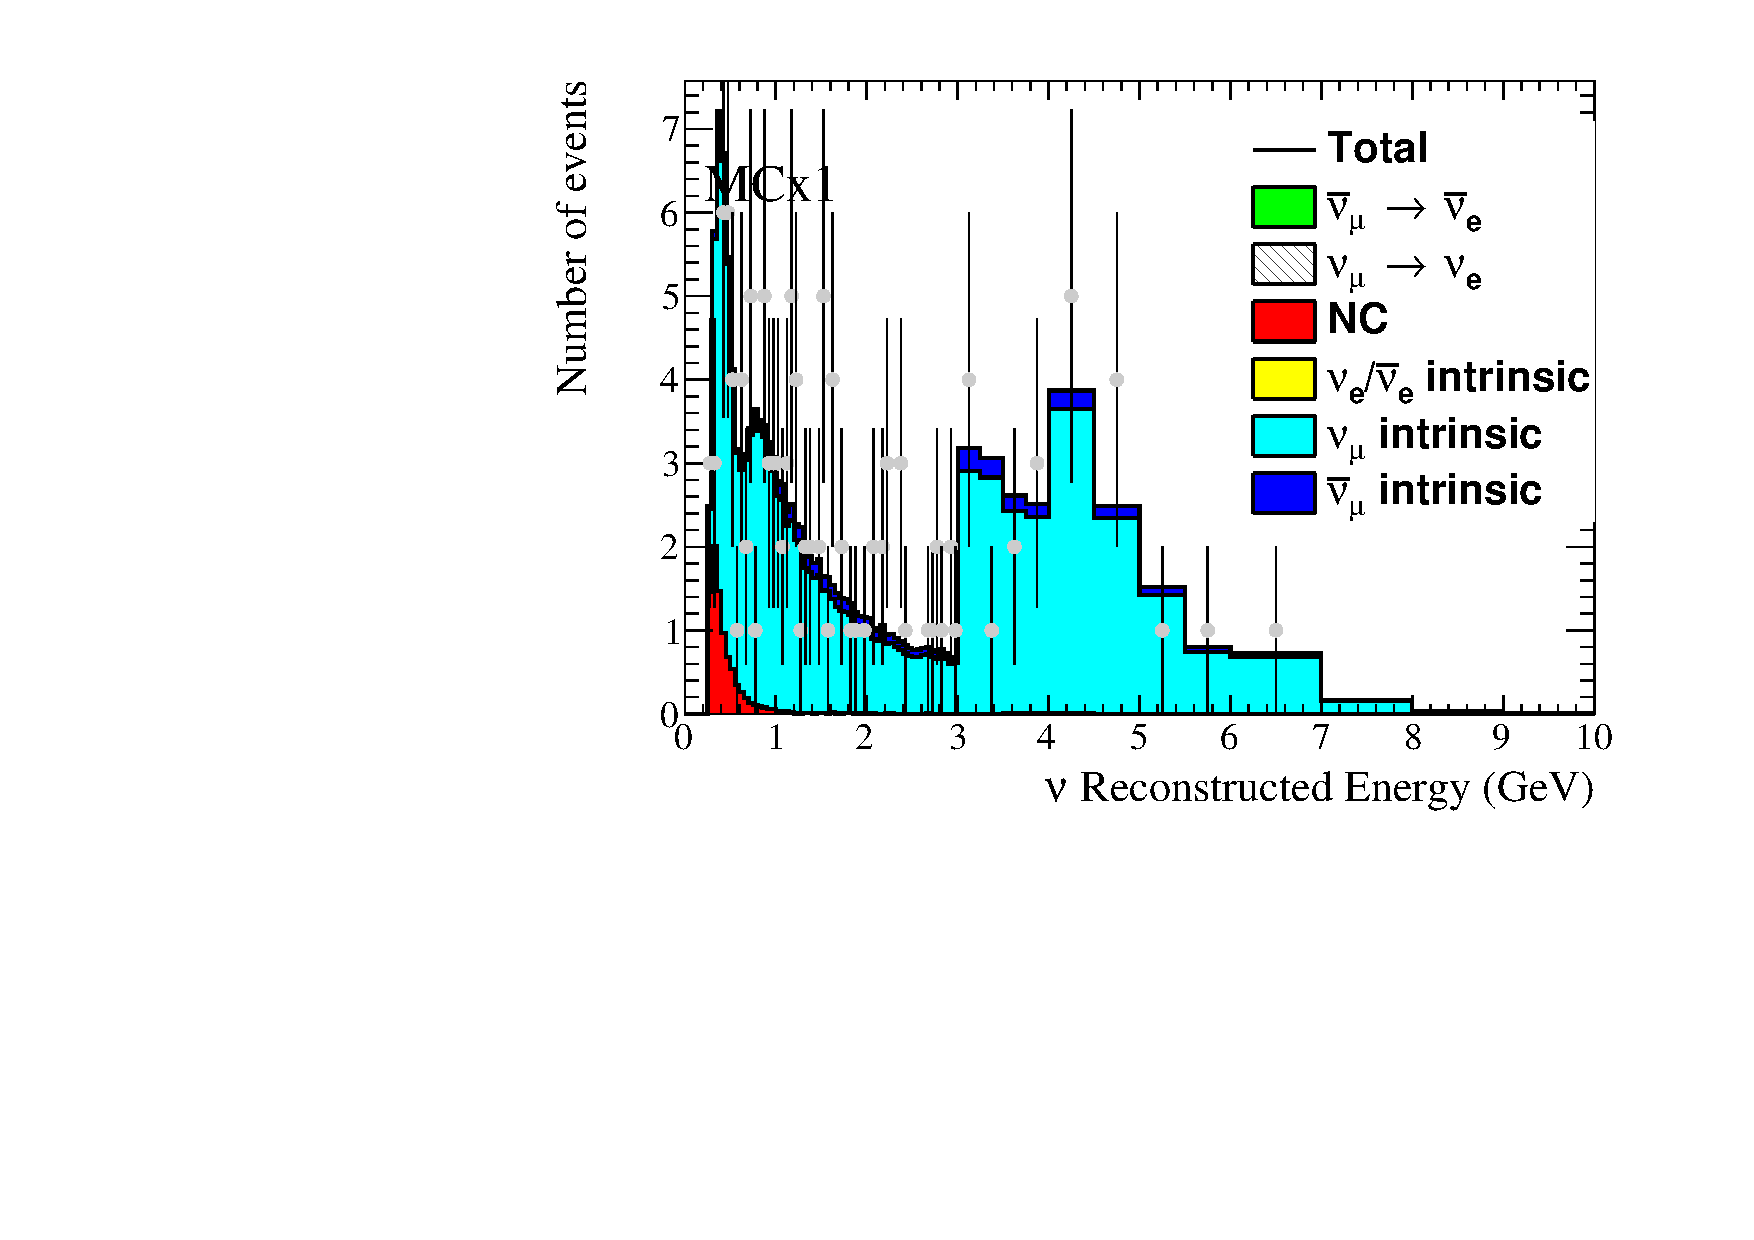
\includegraphics[width=0.9\textwidth]{./joint_plots/data/ccpi/cErecoTotFlavMode_1Rmu.pdf} 
\caption{Muon-like, neutrino mode}
\end{subfigure}
\begin{subfigure}[b]{0.49\textwidth}
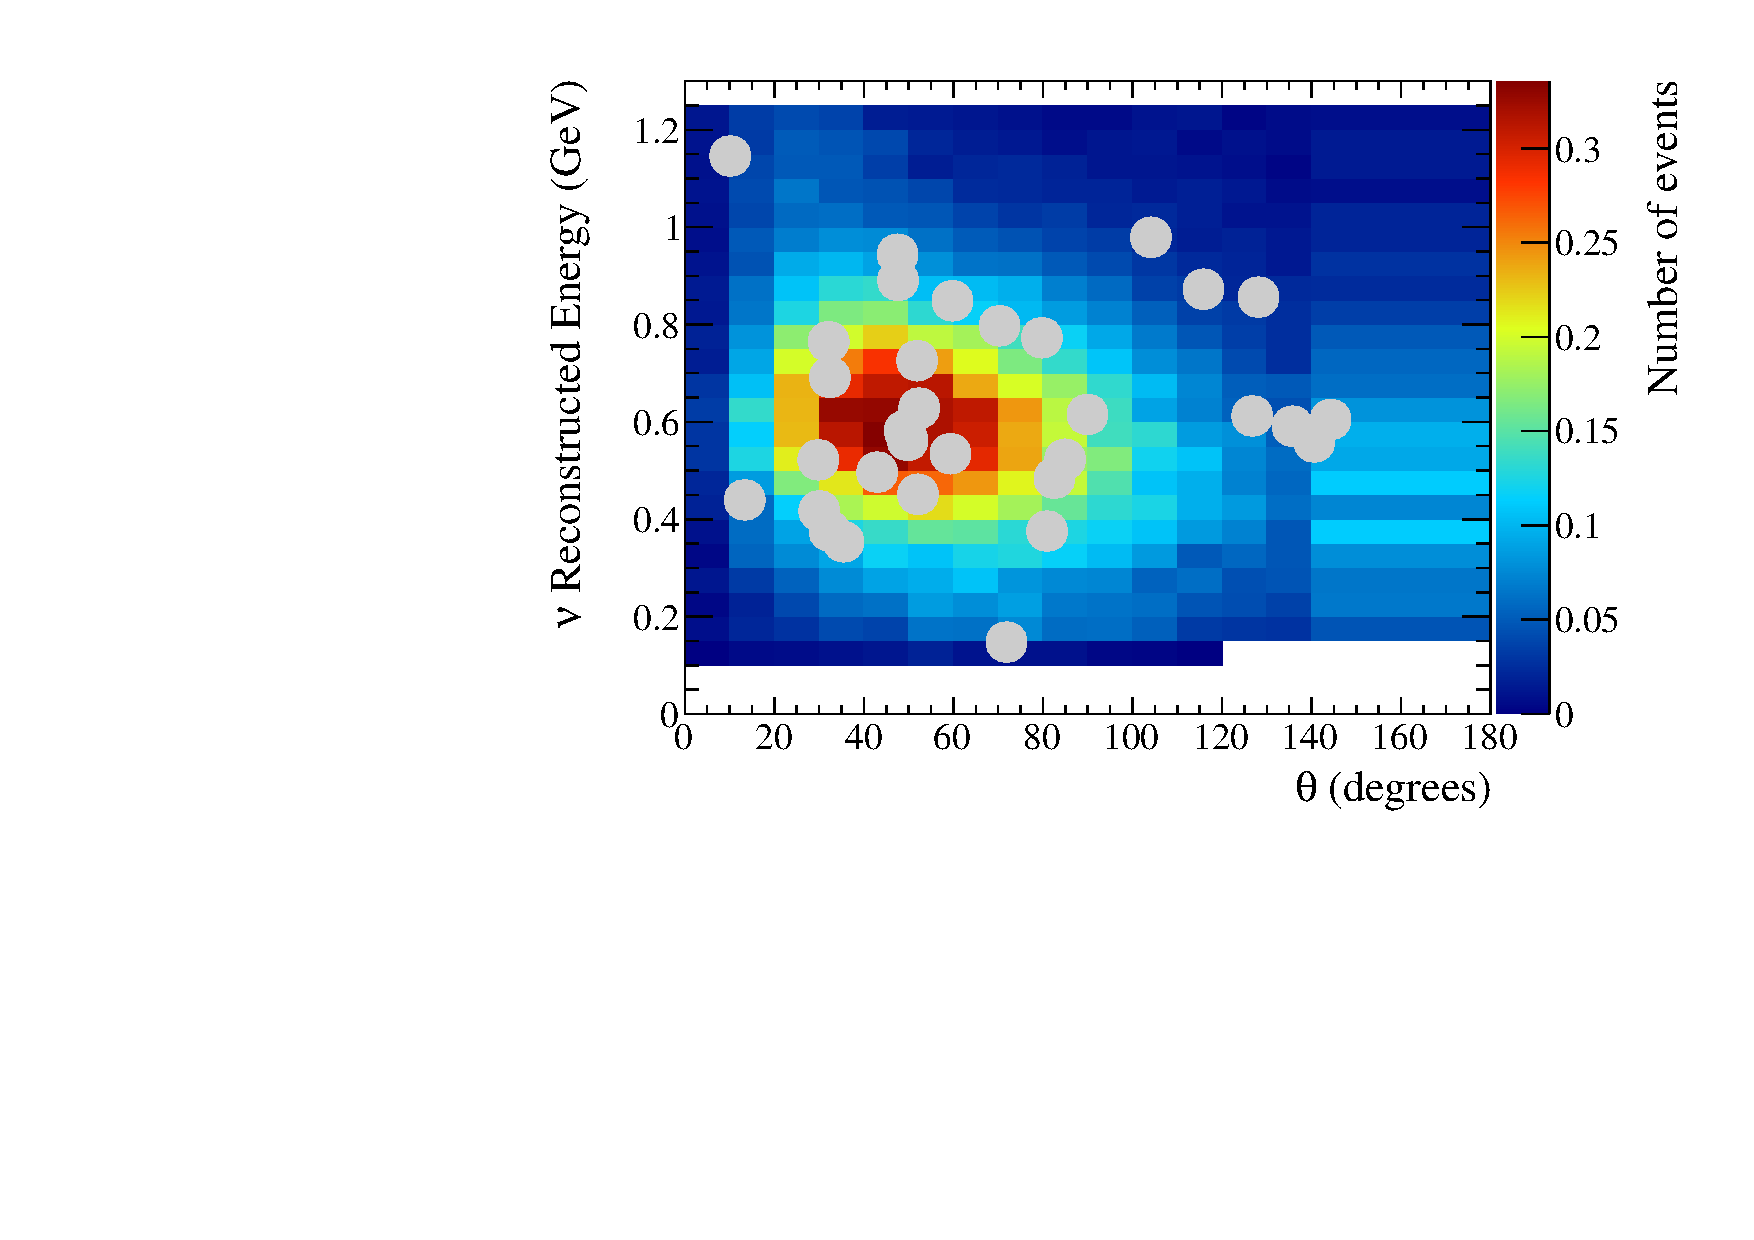
\includegraphics[width=0.9\textwidth]{./joint_plots/data/ccpi/cErecoVsQ2Tot_1Re.pdf} 
\caption{Electron-like, neutrino mode}
\end{subfigure}
\begin{subfigure}[b]{0.49\textwidth}
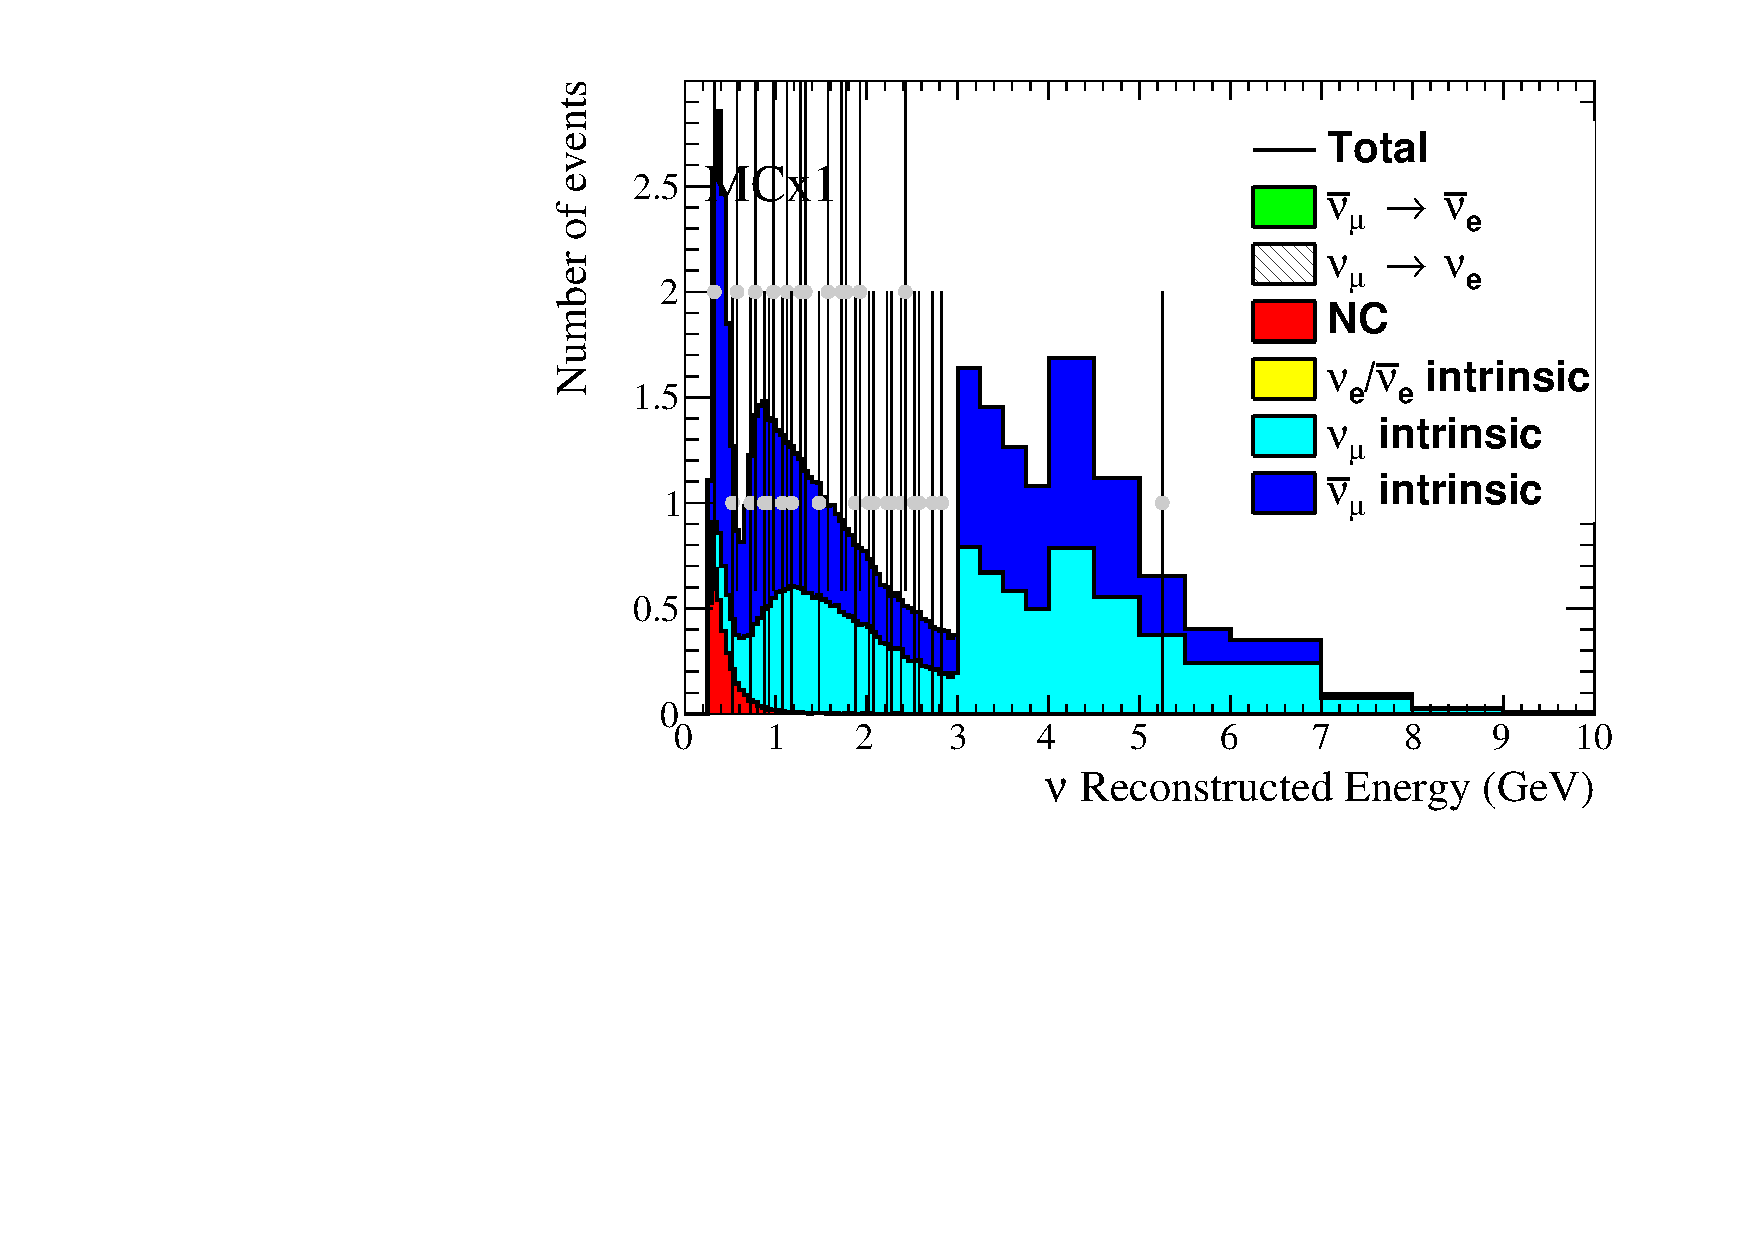
\includegraphics[width=0.9\textwidth]{./joint_plots/data/ccpi/cErecoTotFlavMode_RHC1Rmu.pdf} 
\caption{Muon-like, antineutrino mode}
\end{subfigure}
\begin{subfigure}[b]{0.49\textwidth}
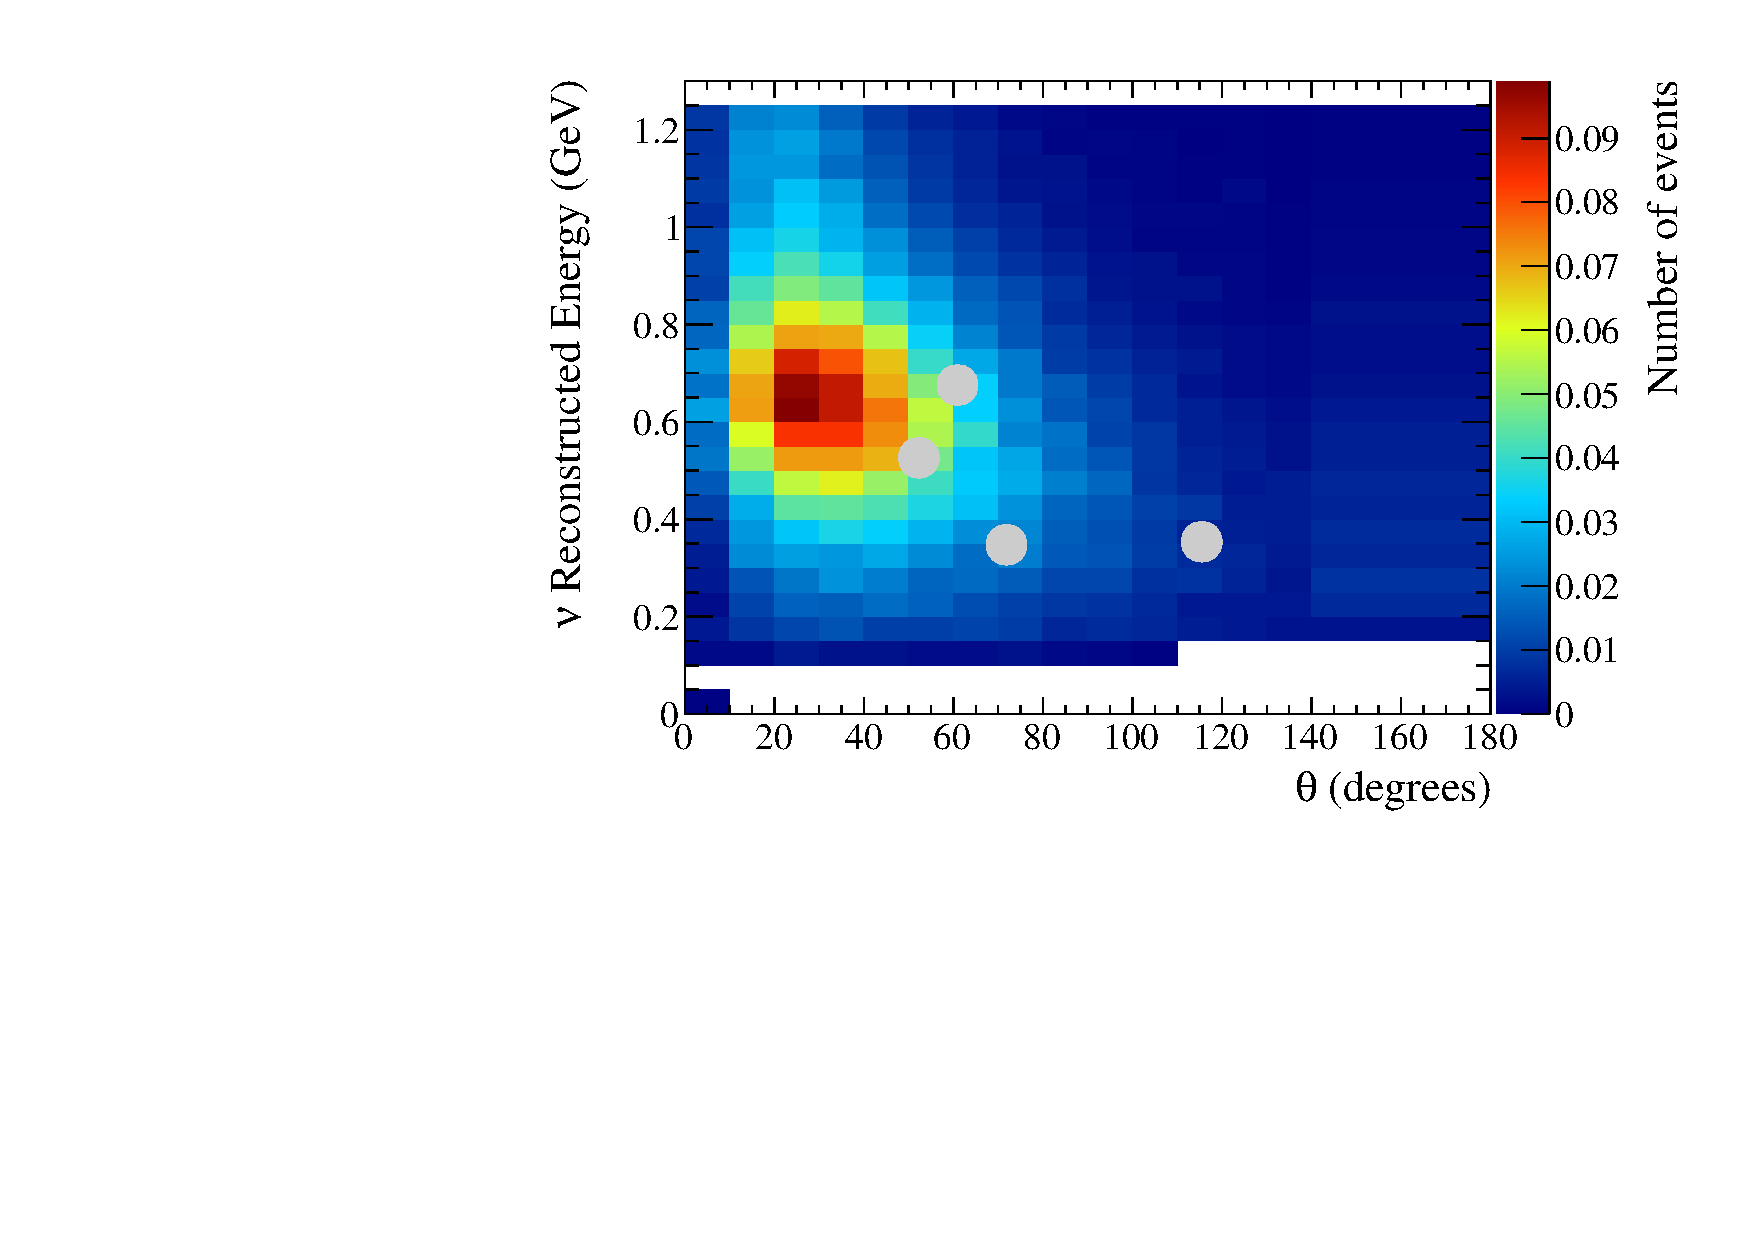
\includegraphics[width=0.9\textwidth]{./joint_plots/data/ccpi/cErecoVsQ2Tot_RHC1Re.pdf} 
\caption{Electron-like, antineutrino mode}
\end{subfigure}
\begin{subfigure}[b]{0.49\textwidth}
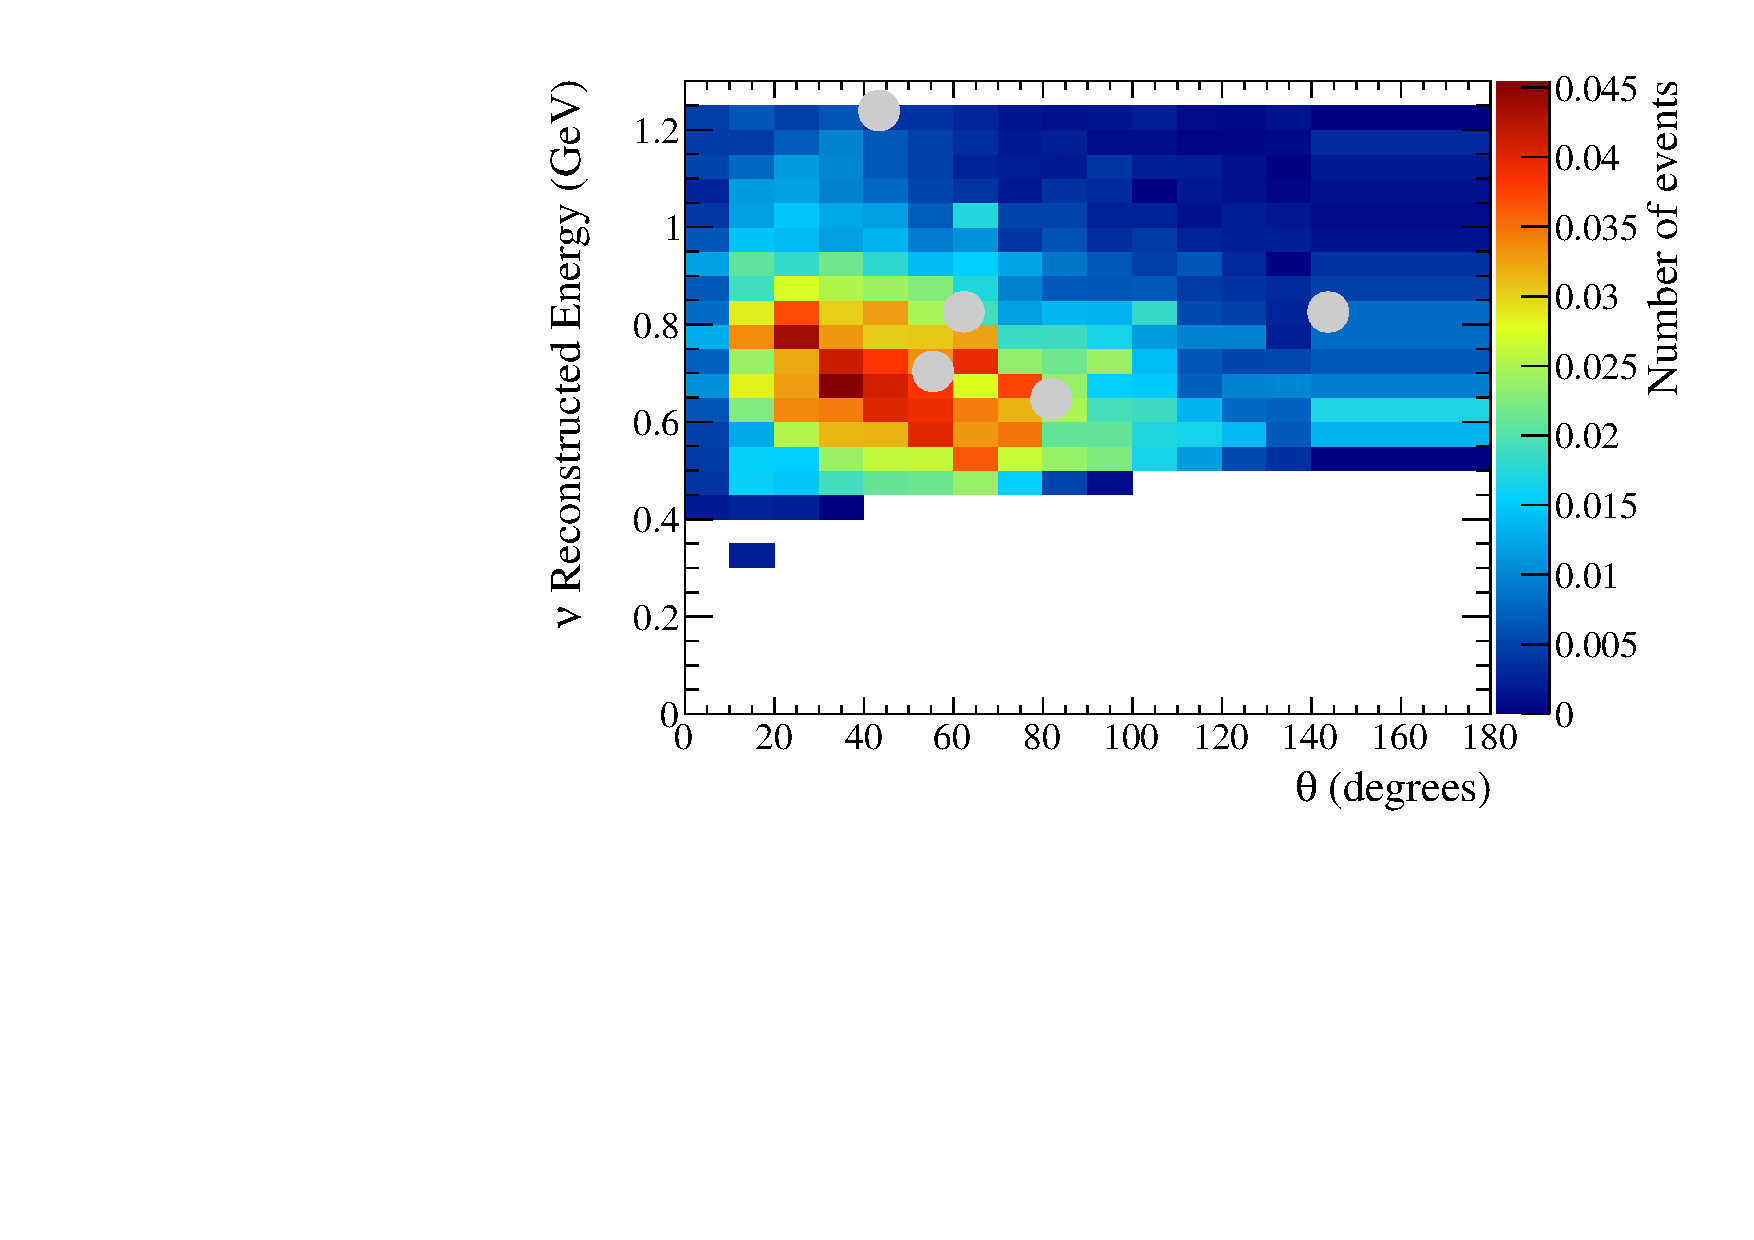
\includegraphics[width=0.9\textwidth]{./joint_plots/data/ccpi/cErecoVsQ2Tot_MultiRe.pdf} 
\caption{cc$\pi^+$-like, neutrino mode}
\end{subfigure}
\caption {
The predicted spectra compared to the Run 1-7c dataset (dots),
which corresponds to an exposure 
of \TotalPotNuRunOneSevenC POT in neutrino mode
and
of \TotalPotNuBarRunOneSevenC POT in antineutrino mode,
are shown.
The expected distribution corresponds to the oscillation parameters of the Asimov data set A shown in \cref{tab:osc_params_joint_asimov}.
The spectra were generated with the systematic parameters measured with the ND280 data 
shown in \cref{tab:banff_uncertainties_flux_fhc},~\ref{tab:banff_uncertainties_flux_rhc},
~\ref{tab:banff_uncertainties_xsec} 
and the nominal Super-K systematic parameters shown in \cref{tab:banff_uncertainties_skdetfsi}.
}
\label{fig:spectra_expVsdata_asimov_A_run17c}
\end{figure}




% Table summarizing the # of observed events in Run 1-6

\begin{table}[htb]
\centering
\begin{tabular}{| c | c | c | c | c | c | c | c |}
\hline
Beam mode	& Sample		& Exp. Asimov A  	& Exp. Asimov A	& Exp. Asimov B	& Exp. Not Osc			& Observed 	& Best fit\\
			& 			& 			  	& ($\delta_{CP}=0$)	& 				& 					& 		 	& (reactors) \\
\hline
neutrino	 	& $\mu$-like 	&135.815			& 135.459			& 140.724	 		& 521.777				& 135 		& 135.255 \\
neutrino 		& $e$-like  	& 28.687 			& 24.170			& 21.524			& 6.147				& 32 			& 28.880 \\
antineutrino 	& $\mu$-like 	& 64.205			& 64.059			& 65.597			& 184.837				& 66 			& 63.870 \\
antineutrino 	& $e$-like 	& 6.004			& 6.902			& 6.252			& 2.335				& 4 			& 6.114 \\
neutrino 		& cc$\pi^+$-like & 3.126 			& 2.744			& 2.511			& 3.258				& 5 			& xxxx \\

\hline
\end{tabular}
\caption{
The observed, expected and best-fit number of events in Run 1-7c data set
for an exposure
of \TotalPotNuRunOneSevenC POT in neutrino mode
and
of \TotalPotNuBarRunOneSevenC POT in antineutrino mode
are shown 
for each selected sample.
The prediction is produced using the BANFF tuning
and the oscillation parameters shown in \cref{tab:osc_params_joint_asimov}.
The total number of events of the best-fit spectra is obtained by using \cref{eq:bestfit_spectrum_marg}.
}
\label{tab:num_events_run17c}
\end{table}













%--------------------------------------------------------------------------------------
%
% 1-dimensional chisq & best-fit
%
%--------------------------------------------------------------------------------------

\subsection {1-dimensional $\chi^2$ distributions and best-fit}
\label{sec:chisq_1d_run17c}


% 1-dimensional contours

1-dimensional $\chi^2$ distributions as in \cref{sec:sensi} are produced
and shown in \cref{fig:joint_data_fit_1d_run17c}.
The best-fit value of $\delta_{CP}$ when the reactor constraint is applied is -1.728
similar to that of the 1Ring sample analysis.
%, i.e. -1.854 (see \cref{tab:joint_bestfit}), but closer to $-\pi/2$ (i.e. -1.571).
 

\begin{figure*}[htb]
\center
\begin{subfigure}[b]{0.49\textwidth}
\includegraphics[width=0.9\textwidth]{joint_plots/data_contours/Run17c/1D/dcp_reactor.pdf}
\caption{$\delta_{CP}$ with reactor constraint}
\label{fig:dcp_fit_with_reactor_data}
\end{subfigure}
\begin{subfigure}[b]{0.49\textwidth}
%
\includegraphics[width=0.9\textwidth]{./images/missing_plot-eps-converted-to.pdf}
\includegraphics[width=0.9\textwidth]{joint_plots/data_contours/Run17c/1D/dcp.pdf}
\caption{$\delta_{CP}$ with T2K data only}
\end{subfigure}
\begin{subfigure}[b]{0.49\textwidth}
%
\includegraphics[width=0.9\textwidth]{./images/missing_plot-eps-converted-to.pdf}
\includegraphics[width=0.9\textwidth]{joint_plots/data_contours/Run17c/1D/ss13.pdf}
\caption{$\sin^2 \theta_{13}$ with T2K data only}
\end{subfigure}
\begin{subfigure}[b]{0.49\textwidth}
\includegraphics[width=0.9\textwidth]{joint_plots/data_contours/Run17c/1D/ss23.pdf}
\caption{$\sin^2 \theta_{23}$ with reactor constraint}
\end{subfigure}
\begin{subfigure}[b]{0.49\textwidth}
\includegraphics[width=0.9\textwidth]{joint_plots/data_contours/Run17c/1D/dmsq.pdf}
\caption{$\Delta m^2_{32}$ ($\Delta m^2_{13}$) with reactor constraint}
\end{subfigure}
\caption{
Measured $\Delta \chi^2$ distributions
with the full Run 1-7c data set.
Both normal (red) and inverted (blue) hierarchies are shown. 
The \emph{constant} $\Delta \chi^2$ method is used. %(see \cref{app:method_cl}).
Both normal and inverted hierarchy $\Delta \chi^2$ distributions are shifted with respect to the same global minimum. 
All the oscillation parameters which are not parameters of interest
are marginalised using the prior distributions shown in \cref{tab:marg_binnning}.
The measured $\Delta \chi^2$ distribution as a function of $\sin^2 \theta_{13}$ is compared
with the value given by the global analysis of the reactor measurements,
$\sin^2 \theta_{13} = 0.0219 \pm 0.0012 $
\cite{pdg_2014},
shown by the yellow bar.
}
\label{fig:joint_data_fit_1d_run17c}
\end{figure*}

%
% Neutrino only Vs AntiNeutrino only
%
%In \cref{fig:joint_dcp_nu_nubar}
%the $\chi^2$ distributions as a function of $\delta_{CP}$
%with reactor constraint
%is obtained by 
%running the analysis using either only neutrino 
%or antineutrino mode samples for the Run 1-6 data set,
%in order to check the compatibility of neutrino and antineutrino mode data.
%The result is mainly driven by the excess of the observed number
%of events in $e$-like neutrino mode sample compared to what is expected.
%Though the significance given by the antineutrino mode samples is still low,
%also given by the fact that $\sin^2 \theta_{23}$ is not constrained 
%by the antineutrino mode $\mu$-like sample
%as much as by  
%the neutrino mode $\mu$-like sample,
%it is interesting to note that the antineutrino data also prefer 
%a value of $\delta_{CP}$ close to $-\pi / 2$.
%
%\begin{figure*}[htb]
%\center
%%
\includegraphics[width=0.9\textwidth]{./images/missing_plot-eps-converted-to.pdf}
%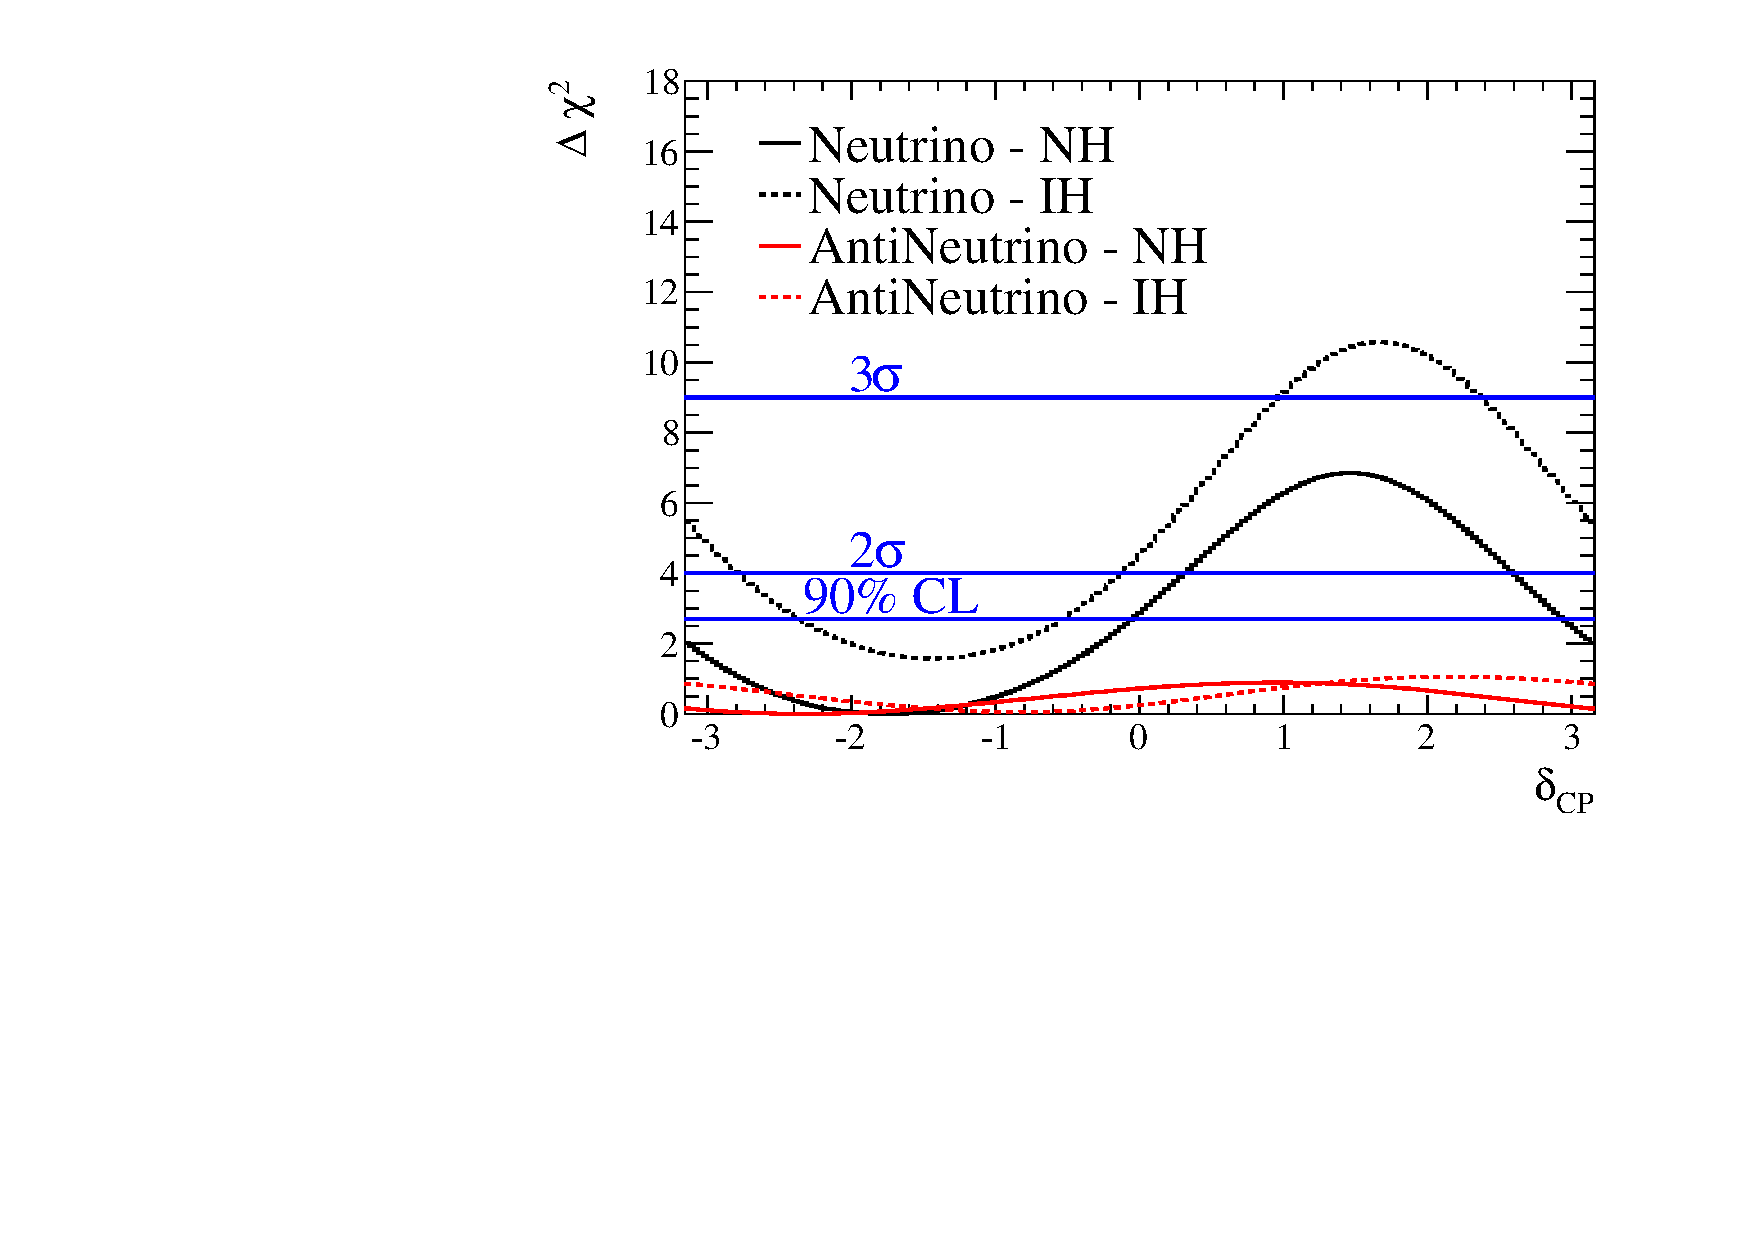
\includegraphics[width=0.5\textwidth]{./joint_plots/data_contours/dcp_react_data_constdchisq_fhcVsrhc.pdf}
%\caption{
%Measured $\Delta \chi^2$ distributions
%with the full Run 1-6 data set
%as a function of
%$\delta_{CP}$ 
%with reactor constraint
%independently for only neutrino and antineutrino mode data.
%Both normal (black) and inverted (red) hierarchies are shown. 
%%Both 68\% (dashed line) and 90\% CL (solid line) are shown.
%%For $\delta_{CP}$ confidence intervals are performed using the
%%\emph{Feldman-Cousins} method,
%%while for the other oscillation parameters
%The \emph{constant} $\Delta \chi^2$ method is used. %(see \cref{app:method_cl}).
%Both normal and inverted hierarchy $\Delta \chi^2$ distributions are shifted with respect to the same global minimum,
%independently for the neutrino and antineutrino mode data. 
%All the oscillation parameters which are not parameters of interest
%are marginalised using the prior distributions shown in \cref{tab:marg_binnning}.
%}
%\label{fig:joint_dcp_nu_nubar}
%\end{figure*}


%
% Rate-only analysis
%
%In \cref{fig:joint_data_fit_1d_rateonly} the $\chi^2$ distributions as a function of $\delta_{CP}$
%is obtained by performing a rate-only analysis; 
%instead of using the shape information of the $E_{reco}$ vs $\theta_l$ spectra,
%the total number of events of each sample is fitted, 
%reducing the $E_{reco}$ vs $\theta_l$ template to 1 bin.
%Then the best-fit value of $\delta_{CP}$ is -1.602 closer to $-\pi/2$ with respect to the case
%where the shape information is used.
%
%\begin{figure*}[htb]
%\center
%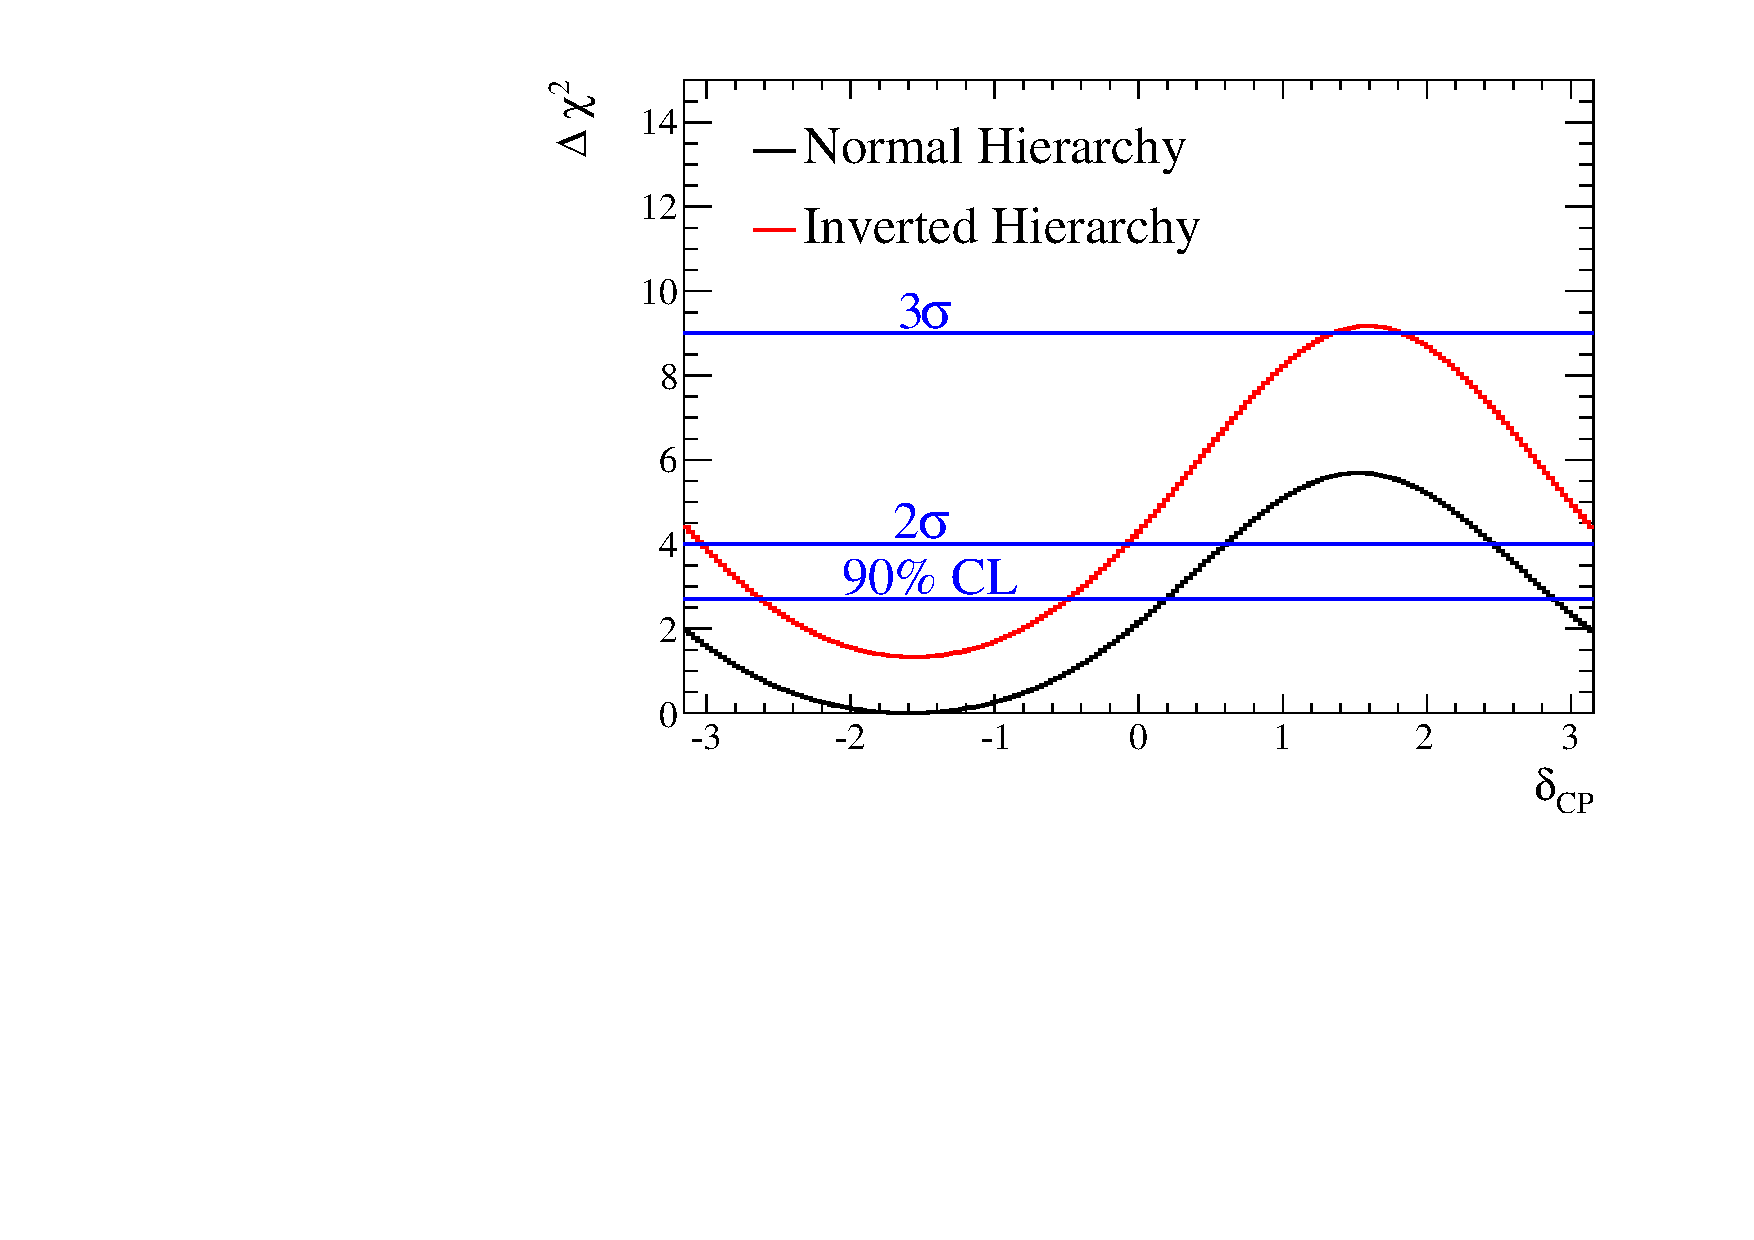
\includegraphics[width=0.5\textwidth]{joint_plots/data_contours/dcp_react_data_constdchisq_rateonly.pdf}
%\caption{
%Measured $\Delta \chi^2$ distributions
%with a rate-only analysis
%using the full Run 1-6 data set
%as a function of
%$\delta_{CP}$ 
%with reactor constraint.
%Both normal (black) and inverted (red) hierarchies are shown. 
%%Both 68\% (dashed line) and 90\% CL (solid line) are shown.
%%For $\delta_{CP}$ confidence intervals are performed using the
%The \emph{constant} $\Delta \chi^2$ method is used. %(see \cref{app:method_cl}).
%Both normal and inverted hierarchy $\Delta \chi^2$ distributions are shifted with respect to the same global minimum. 
%All the oscillation parameters which are not parameters of interest
%are marginalised using the prior distributions shown in \cref{tab:marg_binnning}.
%}
%\label{fig:joint_data_fit_1d_rateonly}
%\end{figure*}




% Table of best-fit and 1sigma ranges

In \cref{tab:joint_bestfit_run17c} the best-fit values as well as the $1\sigma$ ranges for each 
oscillation parameter are shown for the Run 1-7c data fit, for both normal and inverted hierarchy.
The $1\sigma$ ranges are extracted for each oscillation parameter
from the 1-dimensional $\Delta \chi^2$ distributions shown in \cref{fig:joint_data_fit_1d_run17c},
where one oscillation parameter is free and all the other oscillation as well as the systematic 
parameters are marginalised.
The mass hierarchy is minimized:
for both normal and inverted hierarchy the $1\sigma$ ranges are calculated with respect to the 
same global minimum.
Since this approach is not entirely correct and there does not exist any procedure 
to set more reliable confidence intervals which does not consist of toy MC studies (see \cref{sec:cl_mh}),
the advice to the reader is to give more importance to the difference in $\chi^2_{marg}$
between normal and inverted hierarchies in the respective best-fit points, 
instead of the $1\sigma$ ranges of inverted hierarchy, 
which are smaller by construction.
It is also worth to notice that the $1\sigma$ ranges for normal hierarchy (best-fit)
are set correctly with the constant $\Delta \chi^2$ method in the gaussian approximation.

%As already written above, the Run 1-7c best-fit value of $\delta_{CP}$ with reactor constraint is 
%close to the Run 1-6 one (see \cref{tab:joint_bestfit}).
%However if the reactor constraint is not applied, the Run 1-7c best-fit value of $\delta_{CP}$
%is quite different with respect to the Run 1-6 one:
%the best-fit for both normal and inverted hierarchy gets closer to $-\pi/2$.
%Indeed, as shown in \cref{fig:joint_data_fit_1d_run17c}, 
%the $\Delta \chi^2$ distribution as a function of $\delta_{CP}$ and mass hierarchy
%with T2K only data becomes more similar to the one obtained with the reactor constraint:
%assuming the constant $\Delta \chi^2$ method, $\delta_{CP}=0$ for normal hierarchy
%is excluded at 90\%CL and the maximal $\Delta \chi^2$ value is 
%larger than 4.5 and 8.5 respectively for normal and inverted hierarchy.
%The exclusion is stronger than the one given by the Run 1-6 where
%almost the full range $\delta_{CP}$ and normal hierarchy was allowed at 90\%CL.
%This is due to the downward fluctuation in the antineutrino mode $e$-like sample
%combined with an upward fluctuation in the neutrino mode $e$-like sample.
%Assuming Asimov data set A but with $\delta_{CP} = 0$ we expect 6.9
%antineutrino mode $e$-like events and 22.7 neutrino mode $e$-like events.
%If we assume $\delta_{CP}=-1.601$ we expect 26.9 and 6.0 events 
%for neutrino and antineutrino mode $e$-like samples.
%However we observe only 4 events in antineutrino mode and 
%32 events in neutrino mode $e$-like samples.
%Consequently the Run 1-7c data favor a smaller value of $\sin^2 \theta_{13}$,
%in better agreement with the reactor measurement,
%enhancing the tension due to the excess in the neutrino mode $e$-like sample.


%It is interesting to notice that the Run 1-7c $\pm 1\sigma$ interval of $\sin^2 \theta_{23}$ is slightly larger
%than the Run 1-6 one though the number of events in antineutrino mode $\mu$-like samples is almost double. 
%This can be qualitatively understood by comparing the observed and expected number of events
%in \cref{tab:num_events_run17c} (Run 1-7c) and~\ref{tab:num_events} (Run 1-6).
%In Run 1-6 data set the observed number of $\bar{\nu}_{\mu}$ candidates is 34, in good agreement
%with Asimov data set A, i.e. maximal disappearance, while in Run 1-7c data set we observe 66 events
%which is closer to the Asimov data set B, i.e. lower octant ($\sin^2 \theta_{23} = 0.45$).

All the confidence intervals are very similar to those from the 1Ring sample analysis.

\begin{table}[htb]
\centering
\begin{tabular}{| c | c || c | c | c || c | c | c |}
\hline
								& {\bf Reactors}		& \multicolumn{3}{c||}{\bf Normal Hierarchy} & \multicolumn{3}{c|}{\bf Inverted Hierarchy} \\
\hline										
\bf Parameter						&				& Best-fit	& $\chi^2_{min}$	& $\pm 1\sigma$ 	  	 	& Best-fit		& $\chi^2_{min}$ 	& $\pm 1\sigma$ global (inverted) 	 \\
\hline
$\delta_{CP}$             				& YES      			& -1.728  	& 370.61			& [-2.538; -0.877]			& -1.445		& 373.07			& -							\\
								& 				& 		& 				& 						& 			& 				& ([-2.170; -0.768])				\\ 
\hline
$\delta_{CP}$            				& NO        			& -1.791  	& 373.53			& [-2.789; -0.764]			& -1.382		& 375.17			& -							\\
								& 				& 		& 				& 						& 			& 				& ([-2.296;-0.524]) 				\\ 
\hline
$\sin^2 \theta_{13}$    				& NO             		& 0.0271 & 371.44			& [0.0209; 0.0342]			& 0.0299		& 373.38			& -							\\
								& 				& 		& 				& 						& 			& 				& ([0.0232; 0.0380]) 				\\ 
\hline
$\sin^2 \theta_{23}$                      		& YES       		& 0.550	& 369.80			& [0.465; 0.601]			& 0.5525		& 372.30			& -                 					\\
								& 				& 		& 				& 						& 			& 				& ([0.470; 0.601])			  	\\ 
\hline
$\Delta m^2_{32}$ or $\Delta m^2_{13}$   & YES  			& 2.54 	& 369.05	 		& [2.460; 2.621]			& 2.51 		& 297.56			& -     						\\
%								& 				& 		& 				& 						& 			& 				& 				 \\ 
%\hline
($10^{-3} ~\text{eV}^2 / c^4$) 			& 				& 		&				&						&			&				& ([2.429; 2.588])							\\
%								& 				& 		& 				& 						& 			& 				&							 \\ 

\hline
\end{tabular}
\caption{
The Run 1-7c measured oscillation parameter best-fit
and minimum $\chi^2$ 
values  
as well as the 
$1\sigma$ 
CL intervals are shown,
for both normal and inverted hierarchy. 
The $\pm1\sigma$ interval is obtained by using the 
\emph{constant} $\Delta \chi^2$ method.
All the parameters are measured using the reactor constraint 
$\sin^2 2\theta_{13} = 0.085 \pm 0.005 $
\cite{pdg_2014},
except for $\delta_{CP}$ and $\sin^2 \theta_{13}$.
For the inverted hierarchy the intervals are calculated both with respect to 
the global minimum, i.e. normal hierarchy, as well as 
independently for inverted hierarchy (between parenthesis in second row).
As explained in \cref{sec:cl_mh}, the gaussian approximation does not work well 
for discrete parameters like the mass hierarchy however, since there is not a clear way
to compute $1\sigma$ ranges for both mass hierarchies without performing
CPU intensive toy MC studies, the constant $\Delta \chi^2$ method is used.
}                                                                                                                                                                                          
\label{tab:joint_bestfit_run17c}
\end{table}






% Best-fit spectra
{\huge{TO UPDATE}}

The best-fit spectra, shown in \cref{fig:joint_spectra_bf_run17c} are computed as described in \cref{sec:spectra_bestfit_method}
and are compared to the unoscillated nominal spectra.
For $e$-like samples, where 2-dimensional templates are used,
the projection onto the reconstructed neutrino energy axis is shown.
All the systematic and oscillation parameters are marginalised following the procedure described in \cref{sec:spectra_bestfit_method},
while $\sin^2\theta_{23}$, $\delta_{CP}$ and the mass hierarchy were fixed to their best-fit values 
obtained from their simultaneous fit, i.e. \cref{fig:ss23_dcp_with_reactor_data_fit_run17c}.
Indeed these oscillation parameters have the strongest effect on the measurement,
since $\sin^2\theta_{13}$ is constrained with the reactor measurement.

\begin{figure*}[htb]
\center
\begin{subfigure}[b]{0.49\textwidth}
%
\includegraphics[width=0.9\textwidth]{./images/missing_plot-eps-converted-to.pdf}
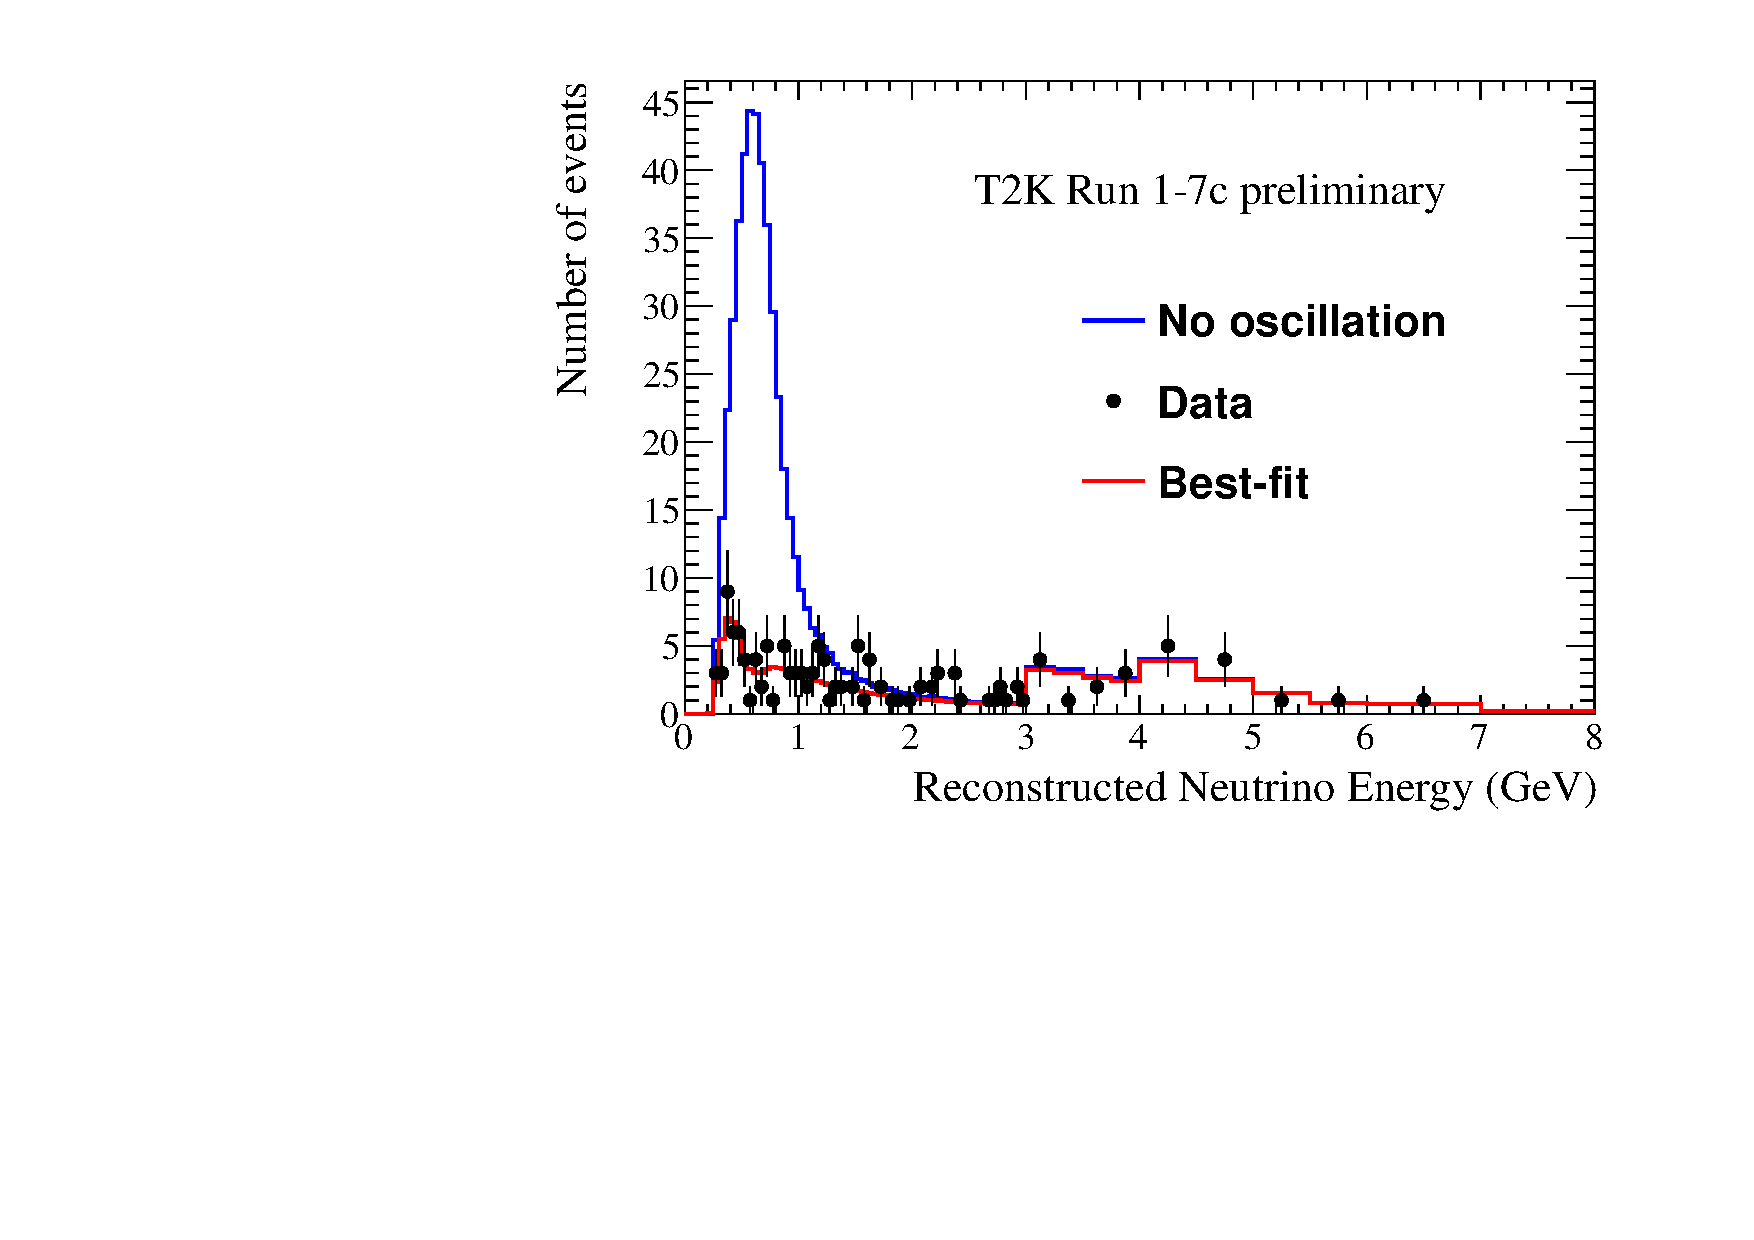
\includegraphics[width=0.9\textwidth]{joint_plots/data/Run17c/bestfit_sinsqth23VsdcpVsMH_1Rmu_Run17.pdf}
\caption{Muon-like, neutrino mode}
\end{subfigure}
\begin{subfigure}[b]{0.49\textwidth}
%
\includegraphics[width=0.9\textwidth]{./images/missing_plot-eps-converted-to.pdf}
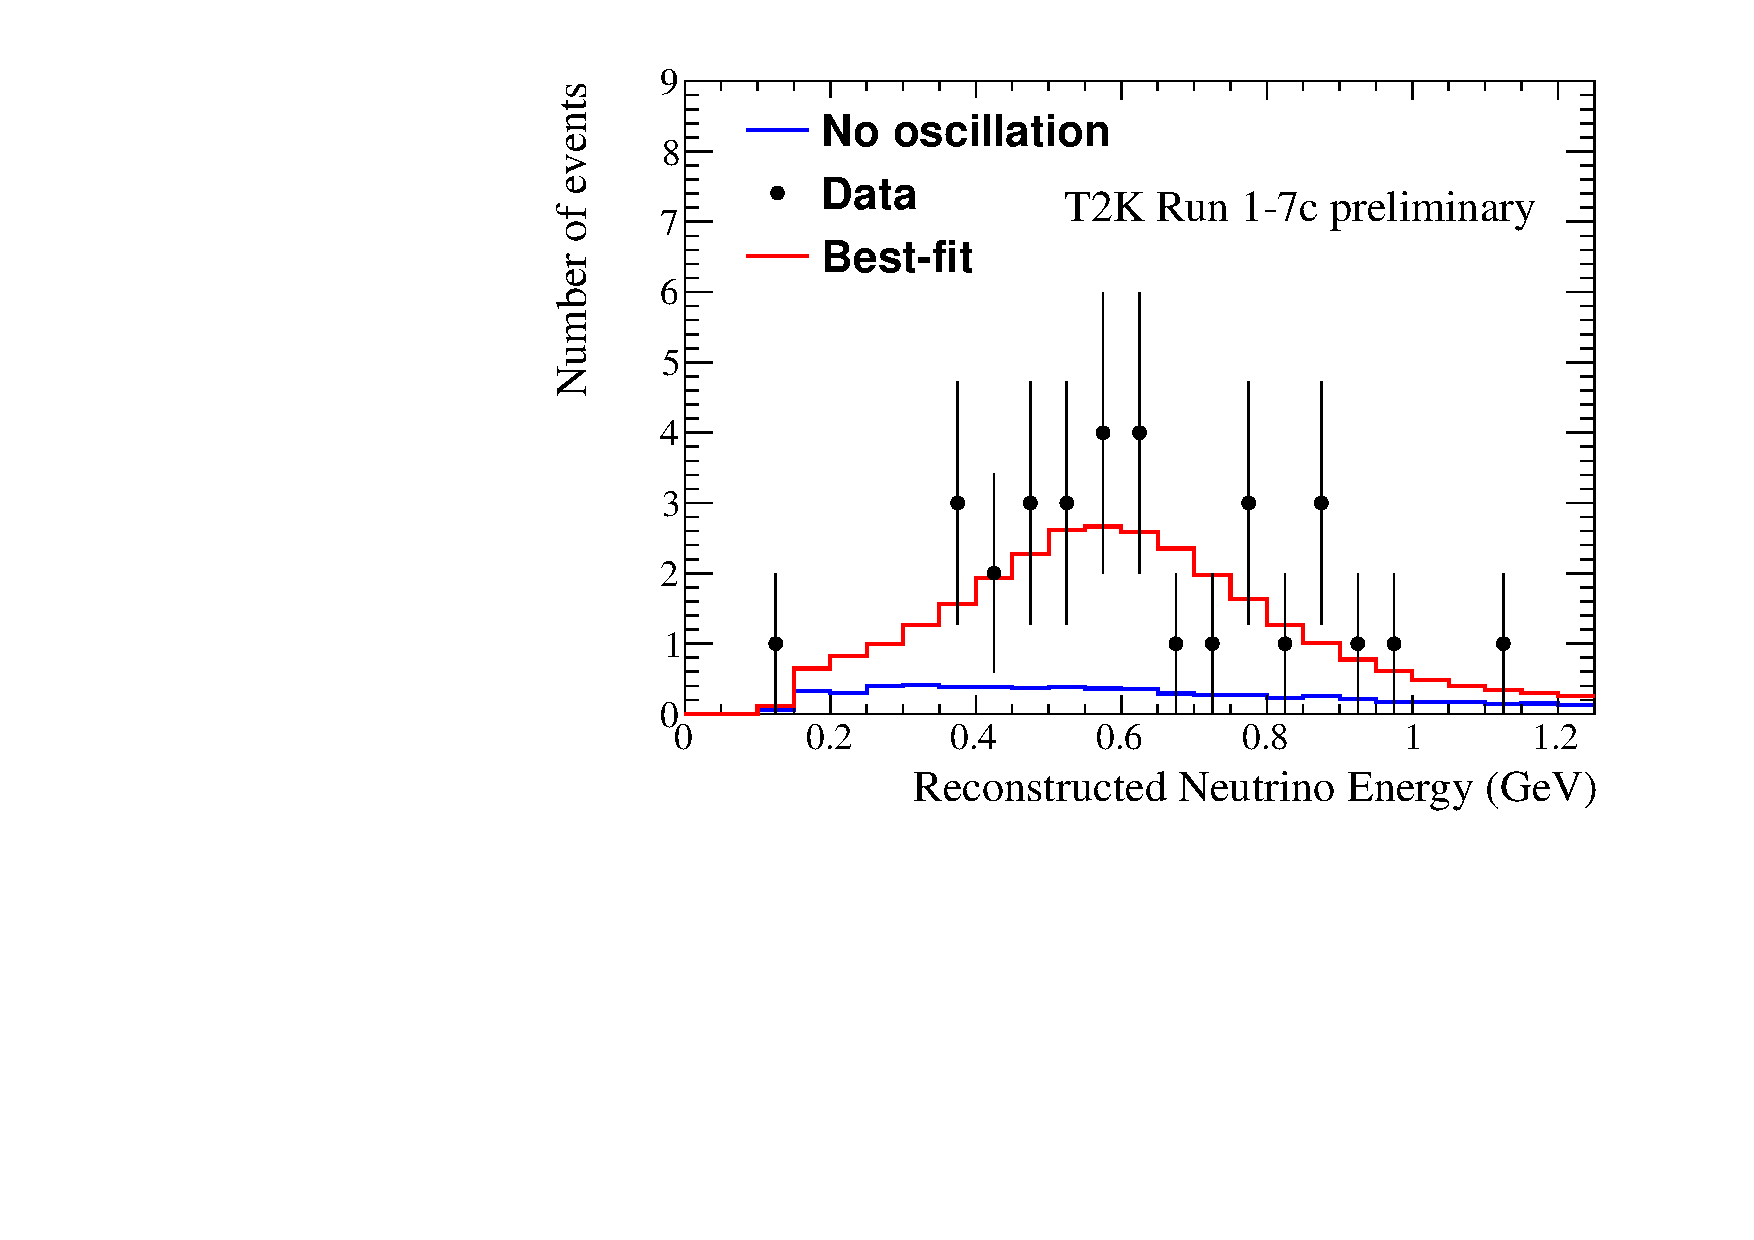
\includegraphics[width=0.9\textwidth]{joint_plots/data/Run17c/bestfit_sinsqth23VsdcpVsMH_1Re_Run17.pdf}
\caption{Electron-like, neutrino mode}
\end{subfigure}
\begin{subfigure}[b]{0.49\textwidth}
%
\includegraphics[width=0.9\textwidth]{./images/missing_plot-eps-converted-to.pdf}
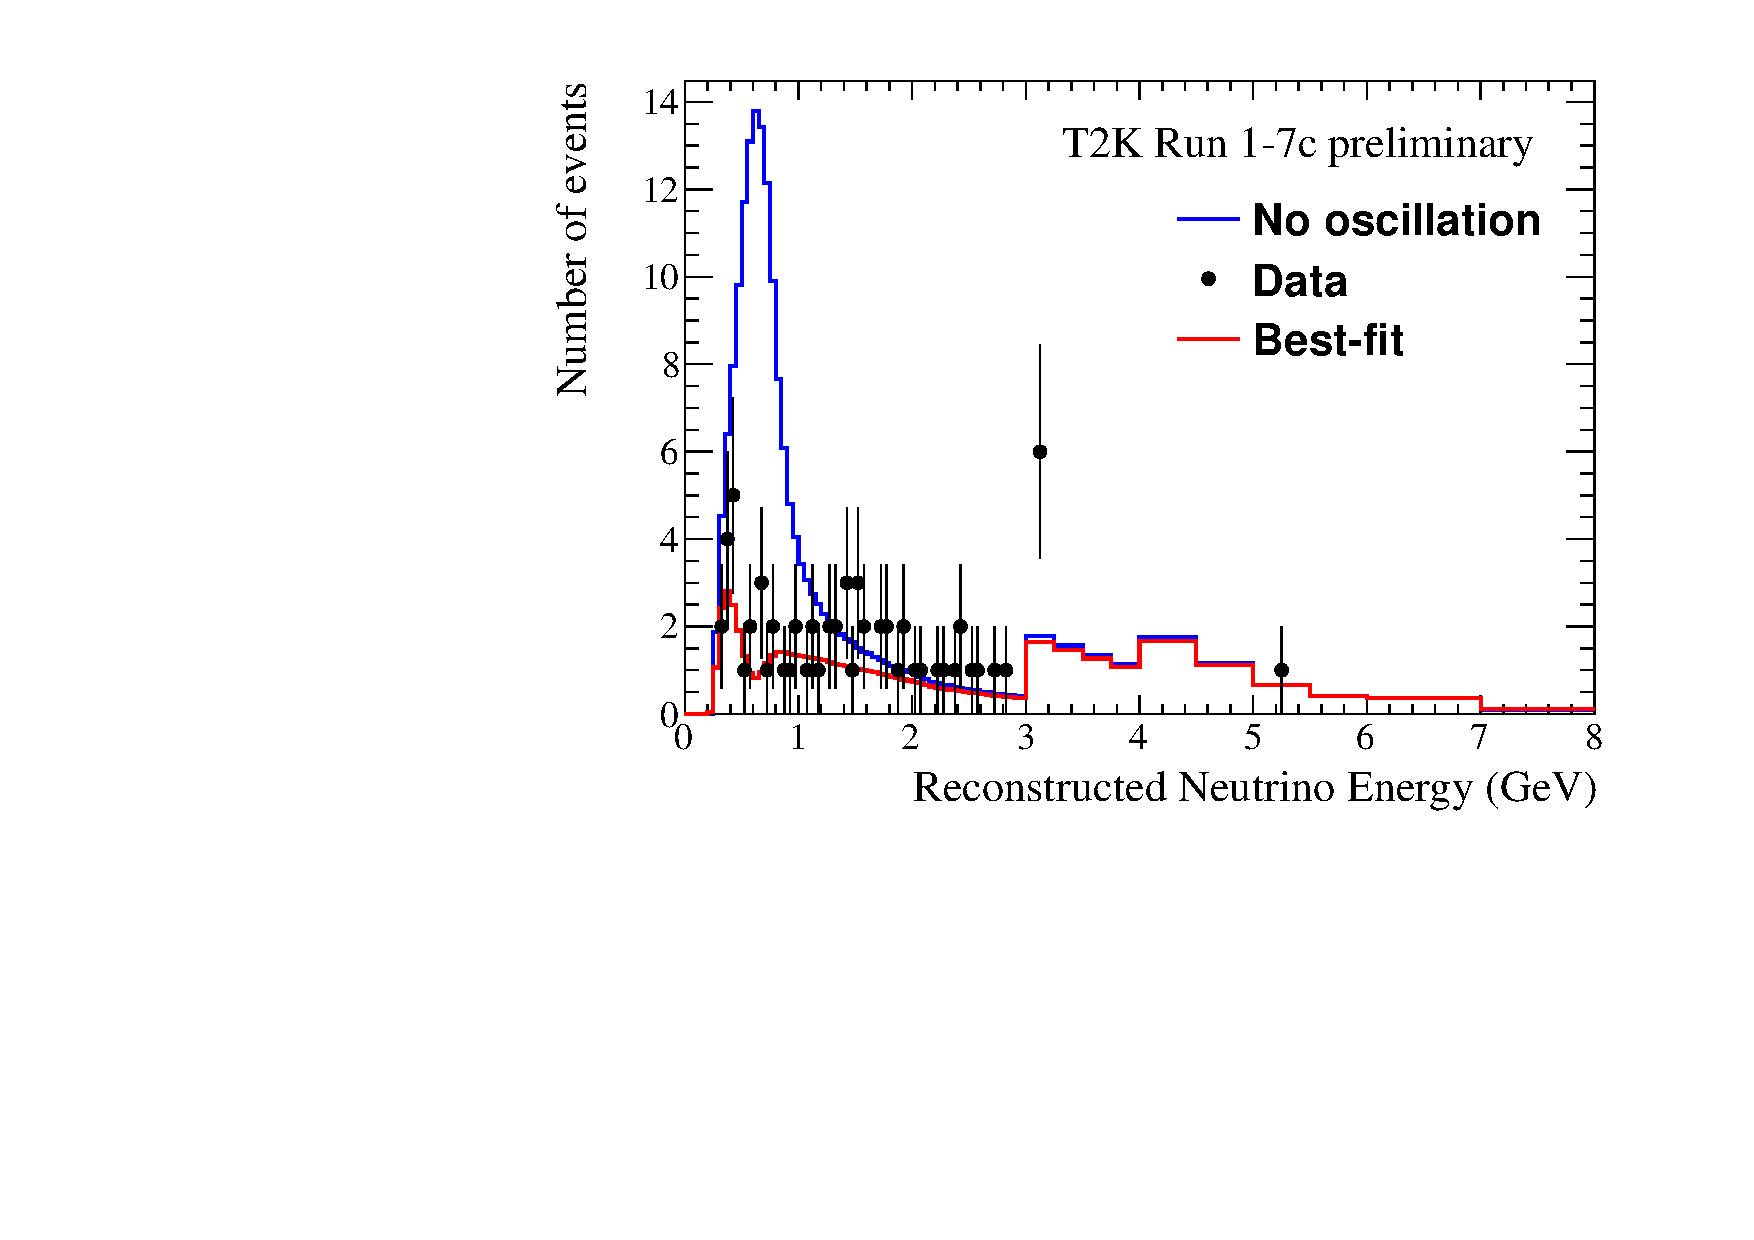
\includegraphics[width=0.9\textwidth]{joint_plots/data/Run17c/bestfit_sinsqth23VsdcpVsMH_RHC1Rmu_Run17.pdf}
\caption{Muon-like, antineutrino mode}
\end{subfigure}
\begin{subfigure}[b]{0.49\textwidth}
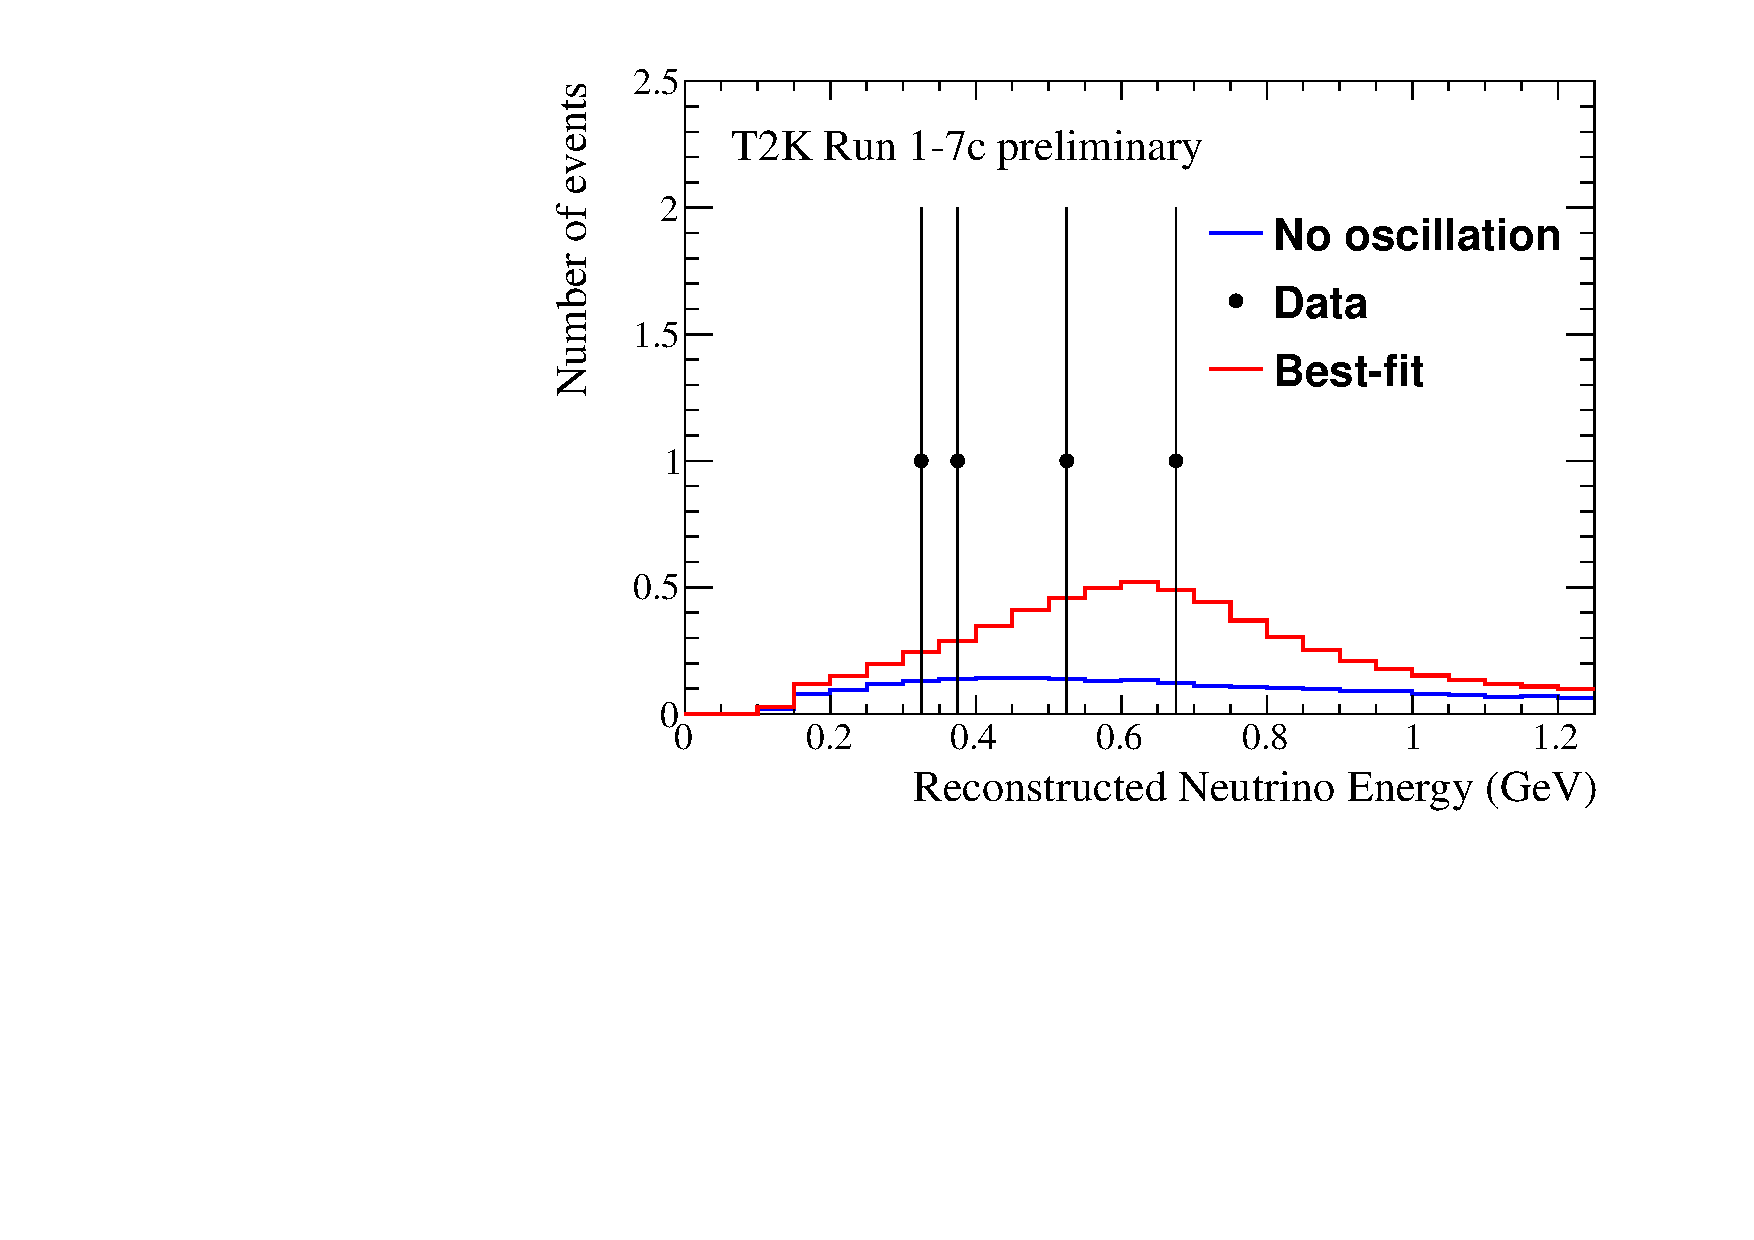
\includegraphics[width=0.9\textwidth]{joint_plots/data/Run17c/bestfit_sinsqth23VsdcpVsMH_RHC1Re_Run17.pdf}
%
\includegraphics[width=0.9\textwidth]{./images/missing_plot-eps-converted-to.pdf}
\caption{Electron-like, antineutrino mode}
\end{subfigure}
\caption {
The best-fit spectra as a function of the neutrino reconstructed energy
are shown for each selected sample
of the Run 1-7c data set.
They correspond to the fit of 
$\sin^2 \theta_{23}$, $\delta_{CP}$ and mass hierarchy 
with reactor constraint
where all the nuisance parameters are marginalised. 
The method described in \cref{eq:bestfit_spectrum_marg} is used.
The best-fit distributions are compared with the 
predicted unoscillated spectrum (all the oscillation parameters are set to 0),
generated with the systematic parameters measured with the ND280 data 
shown in \cref{tab:banff_uncertainties_flux_fhc},
~\ref{tab:banff_uncertainties_flux_rhc},
~\ref{tab:banff_uncertainties_xsec}
and
the nominal Super-K systematic parameters shown in \cref{tab:banff_uncertainties_skdetfsi}.
}
\label{fig:joint_spectra_bf_run17c}
\end{figure*}







% Goodness of fit

A goodness of fit test is performed by comparing data with the best fit spectra shown in \cref{fig:joint_spectra_bf_run17c}.
The same method used for the Run 1-6 and Run 1-7b data sets, shown in \cref{sec:chisq_1d}, is used.
The goodness of fit test has been performed using the same binning as for Run 1-6,
i.e. 5 reconstructed neutrino energy bins (0-0.4, 0.4-0.7, 0.7-1.0, 1.0-2.0 and 2.0-30.0 GeV)
for neutrino mode $\mu$-like and 1 bin for all the other Super-K samples, 
as well as using 5 bins with the same binning as above for both the $\mu$-like samples,
since the antineutrino mode $\mu$-like sample has double of the statistic with Run 1-7c.
At least 6 events are present in each bin.

The $\chi^2$ and resulting p-value for each spectrum is shown in \cref{tab:goodness_of_fit_run17c}. 
We see for all the spectra, the data and best fit spectra are very compatible.

\begin{table}[htb]
\centering
\begin{tabular}{| c | c | c | c |}
\hline
\multicolumn{3}{| c |}{1 bin antineutrino mode $\mu$-like sample}  \\
\hline
Mass Hierarchy d.o.f. 			& $\chi^2$ / ndf        		& p-value \\ \hline
fixed					 		& 2.37348 / 6                  	& 0.88	\\ \hline
free					 		& 2.37348 / 5                 	& 0.80	\\ \hline
\hline
\multicolumn{3}{| c |}{5 bins antineutrino mode $\mu$-like sample}  \\
\hline
Mass Hierarchy d.o.f. 			& $\chi^2$ / ndf        		& p-value \\ \hline
fixed					 		& 3.80457 / 10                  	& 0.96	\\ \hline
free					 		& 3.80457 / 9                 	& 0.92	\\ \hline
\end{tabular}
\caption{
Goodness of fit for the Run 1-7c fit of $\sin^2 \theta_{23}$, $\delta_{CP}$ and mass hierarchy 
where all the other parameters are marginalised. 
Since the mass hierarchy is a discrete parameter, the goodness of the fit test 
is performed assuming the mass hierarchy both as a free parameter and as a fixed parameter.
$ndf = 5$ if the mass hierarchy is assumed to behave as 1 degree of freedom.
The test is performed with both 1 and 5 reconstructed neutrino energy bins for 
antineutrino mode $\mu$-like sample.
}
\label{tab:goodness_of_fit_run17c}
\end{table}



%%--------------------------------------------------------------------------------------
%%
%% Feldman-Cousins deltaCP Vs mh
%%
%%--------------------------------------------------------------------------------------
%
\subsection {Feldman-Cousins and significance for the simultaneous fit of $\delta_{CP}$ and mass hierarchy for Run 1-7c}
\label{sec:fc_significance_run17c}
{\huge{Update}}
%
%
%In \cref{fig:joint_dcp_fc_run17c} the confidence intervals obtained with the ``Feldman-Cousins" method
%are shown for $\delta_{CP}$ and mass hierarchy with reactor constraint for the Run 1-7c data set.
%The critical values at both 90\% and $2\sigma$ CL are computed
%for both the mass hierarchies and the following true values of $\delta_{CP}$: 
%$-\pi$, -2.356, $-\pi/2$, -0.785, 0, +0.785, $+\pi/2$, -2.356, $+\pi$. 
%The procedure described in \cref{sec:cl} is used.
%About 10k toy experiments were used for all the true points except $\delta_{CP} = \pi$ - normal hierarchy.
%Indeed the Run 1-7c data $\Delta \chi^2$ value is very close to the 90\% CL critical value, within one standard deviation of the critical value,
%if only 10k toy experiments are used. 
%For this reason, in order to provide a more precise statement about the 
%90\% CL exclusion of $\delta_{CP} = \pi$ - normal hierarchy, about 28k toy experiments are used, 
%so that the data $\Delta \chi^2$ value is outside the $\pm 1 \sigma$ critical value error.
%This can be seen in in \cref{fig:joint_dcp_fc_run17c}
%where the $\pm 1 \sigma$ error on the critical values are shown as well.
%The same procedure used for the Run 1-6 and Run 1-7b data fit, shown in \cref{sec:fc_significance}, is used.
%Inverted hierarchy is almost excluded at 90\% CL except for a small interval around $\delta_{CP} = -\pi / 2$.
%$\delta_{CP} = 0$ is still disfavored with respect to $\delta_{CP} = \pi$, which, however, is excluded at 90\% CL. 
%We can say that CP conservation assuming the PMNS framework is excluded at 90\% CL also for the Run 1-7c data set,
%though the p-value for $\delta_{CP} = \pi$ and normal hierarchy is very close to 0.1. 
%
%\begin{figure*}[htb]
%\center
%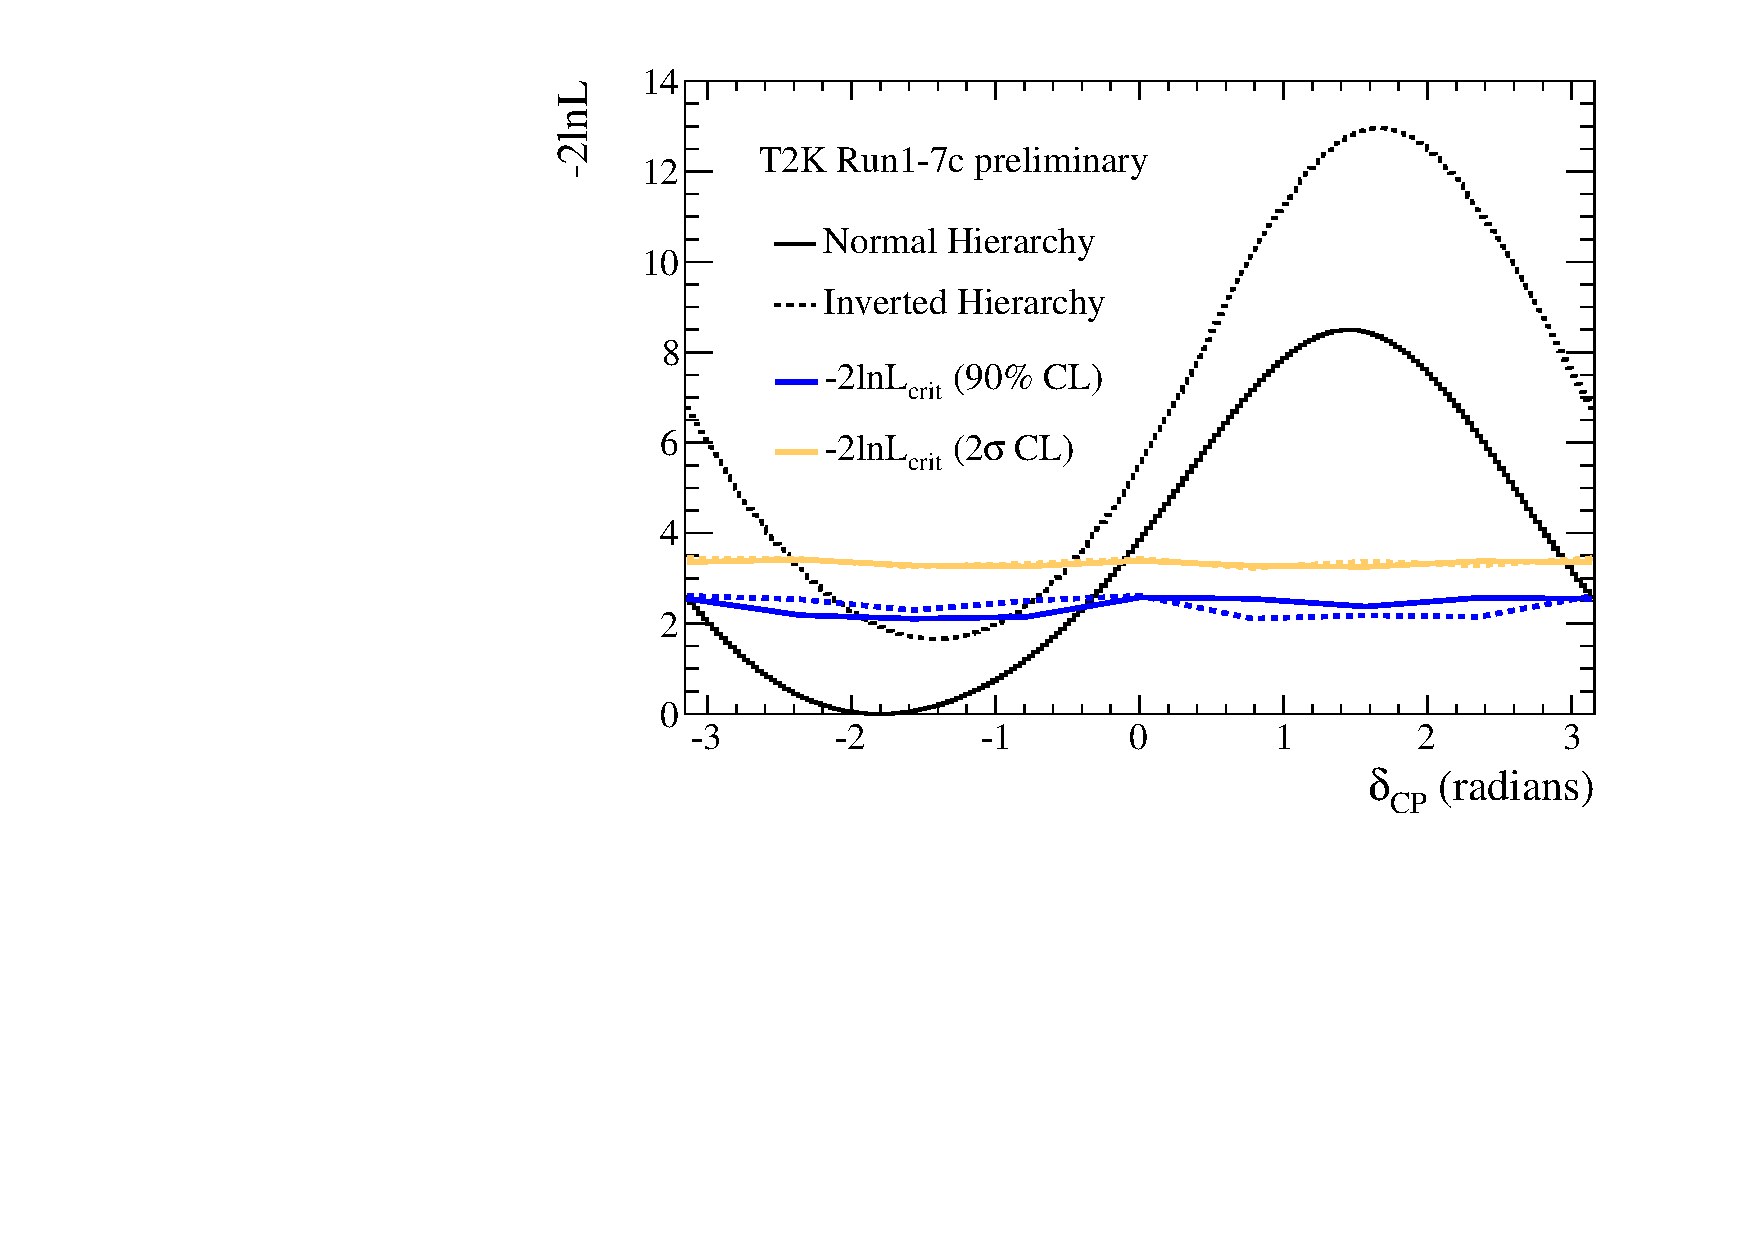
\includegraphics[width=0.49\textwidth]{joint_plots/coverage_fc/fc_run17c/dcp_mh_react_run17.pdf} 
%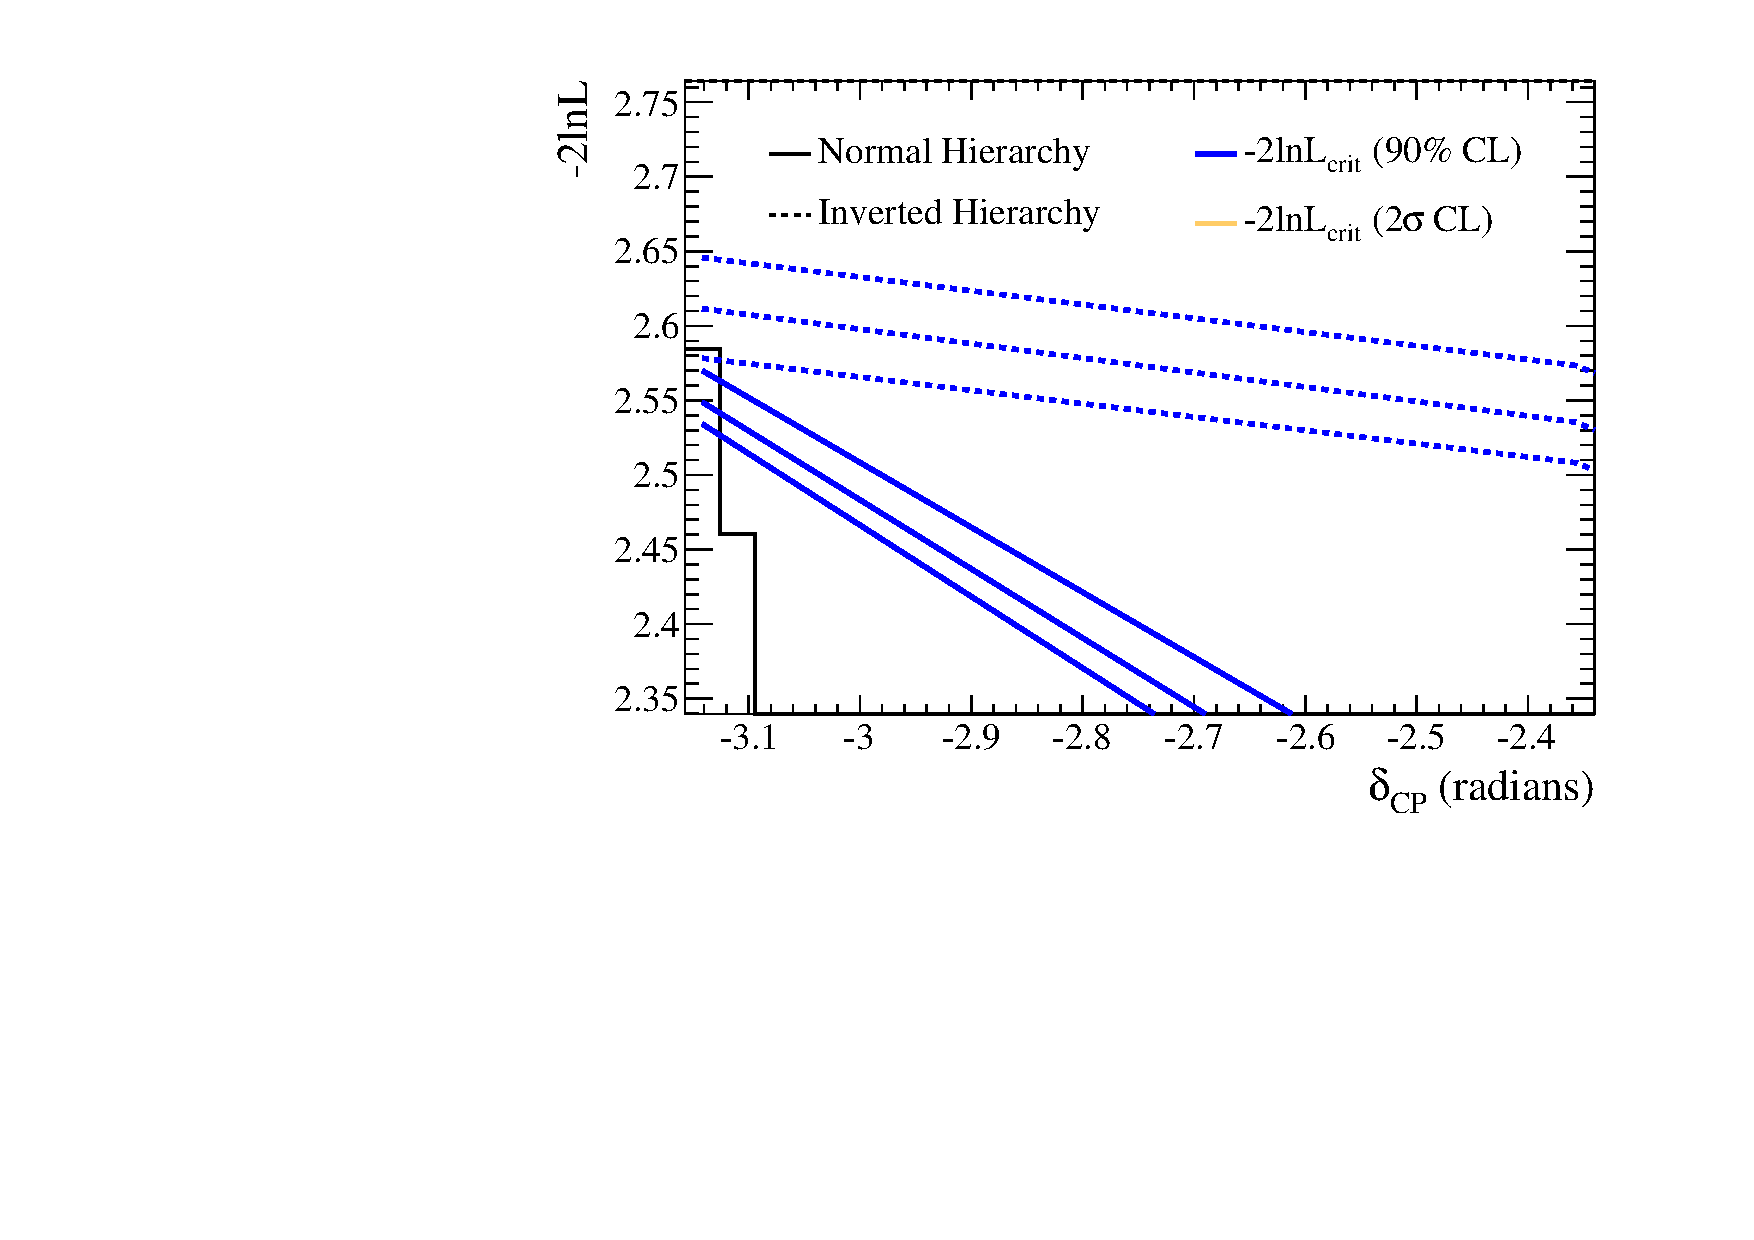
\includegraphics[width=0.49\textwidth]{joint_plots/coverage_fc/fc_run17c/dcp_mh_react_run17_zoom.pdf} \\
%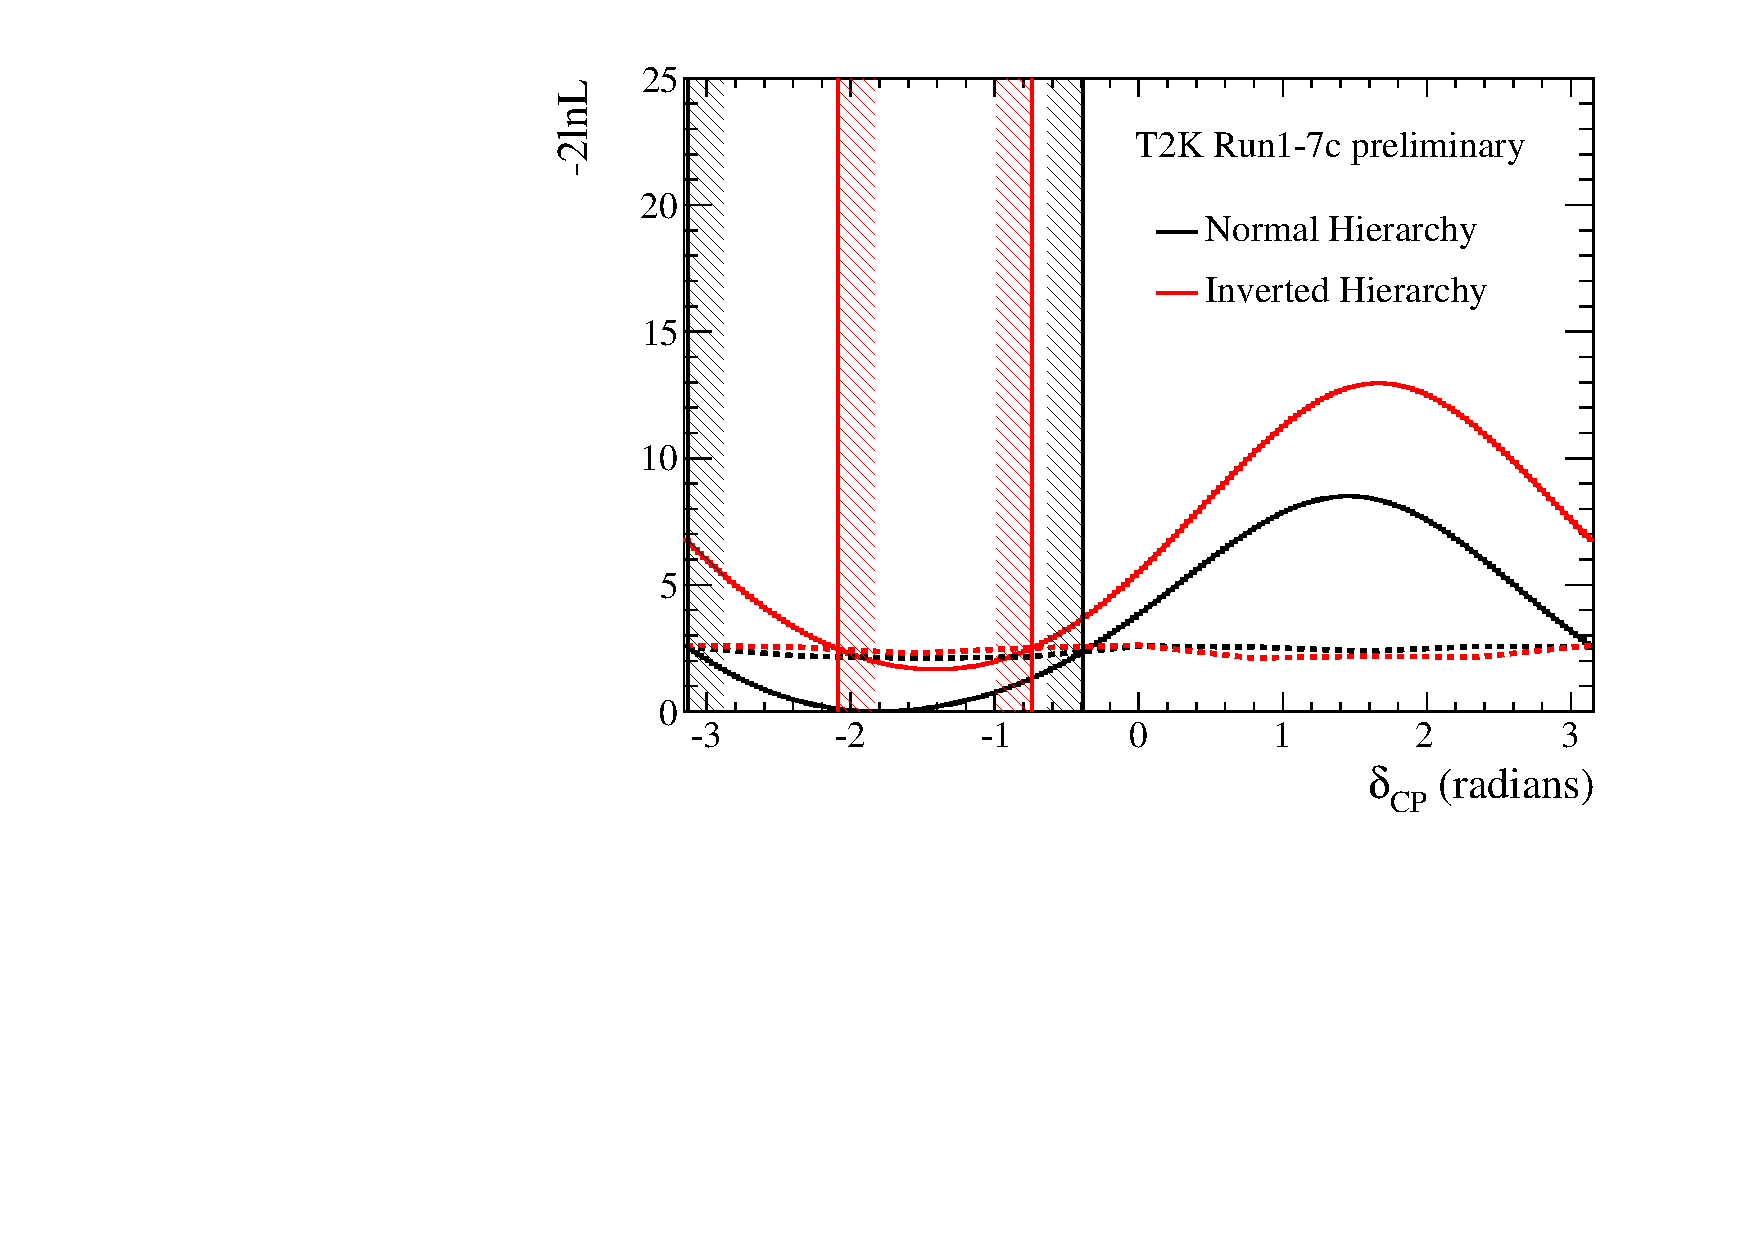
\includegraphics[width=0.49\textwidth]{joint_plots/coverage_fc/fc_run17c/dcp_mh_react_run17_interval_90CL.pdf} 
%\caption{
%Measured $\Delta \chi^2$ distributions with the full Run 1-7c data set.
%Both normal (black solid line) and inverted (black dashed line) hierarchies are shown. 
%The ``Feldman-Cousins" method is used to set the $\Delta \chi^2$ critical values in order to provide 
%confidence intervals with the proper coverage.
%The ranges of $\delta_{CP}$ which correspond to $\Delta \chi^2$ values larger than the critical 
%values (blue for 90\% CL and orange for $2\sigma$ CL) are excluded at a certain confidence level.
%Both normal and inverted hierarchy $\Delta \chi^2$ distributions are shifted with respect to the same global minimum. 
%All the oscillation parameters which are not parameters of interest
%are marginalised using the prior distributions shown in \cref{tab:marg_binnning}.
%The $\pm1 \sigma$ error on the critical values is shown as well, where specified, 
%and is represented by the lowest and highest set of critical values, with the same colour of the central ones.
%On the right plot a zoom on the critical values is shown.
%}
%\label{fig:joint_dcp_fc_run17c}
%\end{figure*}
%
%
%
%In \cref{tab:joint_bestfit_dcp_90CL_interval_FC_run17c} the 90\% CL intervals for $\delta_{CP}$ vs mass hierarchy,
%obtained with the Feldman-Cousins method, are shown.
%
%
%% Interval of deltaCP for 90% CL w/ Feldman-Cousins
%
%\begin{table}[htb]
%\centering
%\begin{tabular}{| c | c | c | c |}
%\hline
%{\bf Parameter}						& {\bf Reactors}		& {\bf Normal Hierarchy}		& {\bf Inverted Hierarchy}		\\
%\hline
%$\delta_{CP}$ (radians) 				& YES      			& [-3.13; -0.39]				& [-2.09; -0.74]				\\
%\hline
%\end{tabular}
%\caption{
%The confidence intervals at 90\% CL obtained with the Feldman-Cousins method
%for the Run 1-7c data set
%is shown for the measurement of $\delta_{CP}$ vs mass hierarchy.
%The reactor constraint $\sin^2 2\theta_{13} = 0.085 \pm 0.005 $ \cite{pdg_2014} is applied.
%}                                                                                                                                                                                          
%\label{tab:joint_bestfit_dcp_90CL_interval_FC_run17c}
%\end{table}
%
%
%\clearpage




















%--------------------------------------------------------------------------------------
%
% Contours
%
%--------------------------------------------------------------------------------------

\subsection {2-dimensional confidence intervals}
\label{sec:results_2d_contours_run17c}

The same 2-dimensional confidence intervals as in \cref{sec:results_2d_contours} are produced.
In \cref{fig:joint_sensi_t2krun14bf_2d_run17c} the corresponding 2-dimensional contours produced
with the Run 1-7c data set are shown drawing the normal and inverted hierarchy contours independently,
i.e. each contour is produced with respect to the global minimum under that hierarchy hypothesis.
In \cref{fig:joint_sensi_t2krun14bf_2d_glob} both normal and inverted hierarchy contours
are produced with respect to the same global minimum, i.e. the normal hierarchy hypothesis.
As already explained in \cref{sec:cl_mh}, ``global" and ``independent" contours correspond
respectively to the least and most conservative approach.

As in 1-dimensional analysis results
in \cref{fig:joint_data_fit_1d_run17c}, the reactor measurements are 
in agreement with the T2K data at $1\sigma$ level if $\delta_{CP} \sim - \frac{\pi}{2}$. 
Compared to \cref{fig:joint_sensi_t2krun14bf_2d}, both the normal and inverted 
hierarchy contours are closer to the reactor measurement.
Furthermore we can see that the region close $\delta_{CP} = + \pi/2$ is excluded at 90\% CL.

In \cref{fig:dcp_run17c_1ring_comparison,2d_reactors_run17c_1ring_comparison,fig:2d_t2konly_run17c_1ring_comparison}
we see the comparison of the results from the 1Ring only analysis with the 1Ring+\nueCConepi{} analysis. The improvement in the
constraints are comparable to the results from the sensitivity study comparison shown in \cref{sec:sensi_run17c}. The constraint 
on $\delta_{cp}$ is slightly stronger than expected which is due to the upward fluctuation observed in the \nueCConepi{} sample 
where 5 events were observed with only 3 expected. With this, there is a noticeably greater exclusion of $\delta_{CP}=\frac{\pi}{2}$.
The effect is also apparent in the $\sin^2 \theta_{13}$ Vs $\delta_{CP}$ contours where the new analysis prefers a larger value
of $\sin^2 \theta_{13}$ which, when constrained by the reactor measurements, results in a stronger constraint on $\delta_{CP}$. 
The comparison of the fits to $\sin^2 \theta_{23}$ Vs $\Delta m^2_{32}$ are slightly unexpected considering the sensitivity study, however the result where a greater portion of the lower octant of $\sin^2 \theta_{23}$ is excluded at 90\%CL and 68\%CL can be explained again by the excess of events observed in the \nueCConepi{}  which favour a much larger value of $\sin^2 \theta_{23}$ and therefore push the parameter to the upper octant. 

%As a result, we see that all $\delta_{CP}$ constraints in 
%\cref{fig:ss13_dcp_with_reactor_data_fit},~\ref{fig:dmsq_dcp_with_reactor_data_fit},~\ref{fig:ss23_dcp_with_reactor_data_fit} 
%are tighter for the inverted hierarchy hypothesis than for the normal.
%\cref{fig:dmsq_dcp_with_reactor_data_fit} also shows a slight anti-correlation between $\delta_{CP}$ 
%and $\Delta m^2_{32}$ in the normal hierarchy fit and a correlation in the inverted most likely coming 
%from the fact that $\Delta m^2_{32}$ and $cos(\delta_{CP})$ have similar effects on the shape of the appearance spectra. 
%In \cref{fig:ss23_dcp_with_reactor_data_fit} we see correlation where the constraint on $\delta_{CP}$ is narrower 
%for smaller values of $\sin^2 \theta_{23}$ as they both appear in the appearance term. 
%In \cref{fig:ss23_dmsq_with_reactor_data_fit} we see that $\sin^2 \theta_{23}$ and $\Delta m^2_{32}$ 
%are not very correlated however the inverted hierarchy contour is shifted down in $\Delta m^2_{32}$ 
%with respect to the normal hierarchy contour. 
%This effect is due to the correlation between $\Delta m^2_{32}$ and the mass hierarchy shown in \cref{fig:mass_hierarchy_MC_shift}. 
%Indeed the inverted hierarchy hypothesis produces an event migration toward higher energy 
%which is balanced in the fit by a lower fit value of $\Delta m^2_{13}$ with respect to the normal hierarchy case.

\begin{figure*}[htb]
\center
\begin{subfigure}[b]{0.49\textwidth}
%
\includegraphics[width=0.9\textwidth]{./images/missing_plot-eps-converted-to.pdf}
\includegraphics[width=0.9\textwidth]{joint_plots/data_contours/Run17c/2D/cp_13.pdf}
\caption{$\sin^2 \theta_{13}$ vs $\delta_{CP}$ with T2K data only}
\label{fig:ss13_dcp_t2k_only_data_fit_run17c}
\end{subfigure}
\begin{subfigure}[b]{0.49\textwidth}
\includegraphics[width=0.9\textwidth]{joint_plots/data_contours/Run17c/2D/cp_13_reactor.pdf}
\caption{$\sin^2 \theta_{13}$ vs $\delta_{CP}$ with reactor constraint}
\label{fig:ss13_dcp_with_reactor_data_fit_run17c}
\end{subfigure}
\begin{subfigure}[b]{0.49\textwidth}
\includegraphics[width=0.9\textwidth]{joint_plots/data_contours/Run17c/2D/dmsq_dcp.pdf}
\caption{$\Delta m^2_{32}$ ($\Delta m^2_{13}$) vs $\delta_{CP}$ with reactor constraint}
\label{fig:dmsq_dcp_with_reactor_data_fit_run17c}
\end{subfigure}
\begin{subfigure}[b]{0.49\textwidth}
\includegraphics[width=0.9\textwidth]{joint_plots/data_contours/Run17c/2D/ss23_dcp.pdf}
\caption{$\sin^2 \theta_{23}$ vs $\delta_{CP}$ with reactor constraint}
\label{fig:ss23_dcp_with_reactor_data_fit_run17c}
\end{subfigure}
\begin{subfigure}[b]{0.49\textwidth}
\includegraphics[width=0.9\textwidth]{joint_plots/data_contours/Run17c/2D/ss23_dmsq.pdf}
\caption{$\sin^2 \theta_{23}$ vs $\Delta m^2_{32}$ ($\Delta m^2_{13}$)
with reactor constraint}
\label{fig:ss23_dmsq_with_reactor_data_fit_run17c}
\end{subfigure}
\caption{
%{\large{MEASURED 2D CONTOURS}}
Measured confidence intervals with the full Run 1-7c data set.
Both normal (black) and inverted (red) hierarchies are shown. 
Both 68\% (dashed line) and 90\% CL (solid line) are shown.
Confidence intervals are produced using the \emph{constant} $\Delta \chi^2$ method. % (see \cref{app:method_cl}).
Contours for normal (black) and inverted (red) hierarchy are computed independently.
All the oscillation parameters which are not parameters of interest
are marginalised using the prior distributions shown in \cref{tab:osc_params_joint_priors}.
The measured contour of $\sin^2 \theta_{13}$ vs $\delta_{CP}$ without reactor constraint, in \cref{fig:ss13_dcp_t2k_only_data_fit} is compared with the measurement by reactor experiments, 
$\sin^2 \theta_{13} = 0.0219 \pm 0.0012 $
\cite{pdg_2014},
shown by the yellow bar.
}
\label{fig:joint_sensi_t2krun14bf_2d_run17c}
\end{figure*}


\begin{figure*}[htb]
\center
\begin{subfigure}[b]{0.49\textwidth}
%
\includegraphics[width=0.9\textwidth]{./images/missing_plot-eps-converted-to.pdf}
\includegraphics[width=0.9\textwidth]{joint_plots/data_contours/Run17c/2D/cp_13_glob.pdf}
\caption{$\sin^2 \theta_{13}$ vs $\delta_{CP}$ with T2K data only}
\label{fig:ss13_dcp_t2k_only_data_fit_run17c}
\end{subfigure}
\begin{subfigure}[b]{0.49\textwidth}
\includegraphics[width=0.9\textwidth]{joint_plots/data_contours/Run17c/2D/cp_13_reactor_glob.pdf}
\caption{$\sin^2 \theta_{13}$ vs $\delta_{CP}$ with reactor constraint}
\label{fig:ss13_dcp_with_reactor_data_fit_run17c}
\end{subfigure}
\begin{subfigure}[b]{0.49\textwidth}
\includegraphics[width=0.9\textwidth]{joint_plots/data_contours/Run17c/2D/dmsq_dcp_glob.pdf}
\caption{$\Delta m^2_{32}$ ($\Delta m^2_{13}$) vs $\delta_{CP}$ with reactor constraint}
\label{fig:dmsq_dcp_with_reactor_data_fit_run17c}
\end{subfigure}
\begin{subfigure}[b]{0.49\textwidth}
\includegraphics[width=0.9\textwidth]{joint_plots/data_contours/Run17c/2D/ss23_dcp_glob.pdf}
\caption{$\sin^2 \theta_{23}$ vs $\delta_{CP}$ with reactor constraint}
\label{fig:ss23_dcp_with_reactor_data_fit_run17c}
\end{subfigure}
\begin{subfigure}[b]{0.49\textwidth}
\includegraphics[width=0.9\textwidth]{joint_plots/data_contours/Run17c/2D/ss23_dmsq_glob.pdf}
\caption{$\sin^2 \theta_{23}$ vs $\Delta m^2_{32}$ ($\Delta m^2_{13}$)
with reactor constraint}
\label{fig:ss23_dmsq_with_reactor_data_fit_run17c}
\end{subfigure}
\caption{
%{\large{MEASURED 2D CONTOURS}}
Measured confidence intervals with the full Run 1-7c data set.
Both normal (black) and inverted (red) hierarchies are shown. 
Both 68\% (dashed line) and 90\% CL (solid line) are shown.
Confidence intervals are produced using the \emph{constant} $\Delta \chi^2$ method. % (see \cref{app:method_cl}).
Contours for normal (black) and inverted (red) hierarchy are computed with respect to the minimum $\chi^2$ 
in both hierarchies.
All the oscillation parameters which are not parameters of interest
are marginalised using the prior distributions shown in \cref{tab:osc_params_joint_priors}.
The measured contour of $\sin^2 \theta_{13}$ vs $\delta_{CP}$ without reactor constraint, in \cref{fig:ss13_dcp_t2k_only_data_fit} is compared with the measurement by reactor experiments, 
$\sin^2 \theta_{13} = 0.0219 \pm 0.0012 $
\cite{pdg_2014},
shown by the yellow bar.
}
\label{fig:joint_sensi_t2krun14bf_2d_run17c_glob}
\end{figure*}


\begin{figure*}[htb]
\center
\begin{subfigure}[b]{0.49\textwidth}
\includegraphics[width=0.9\textwidth]{./joint_plots/data_contours/Run17c/1D_comp/dcp_reactor_nh_a.pdf}
\caption{Normal hierarchy with the reactor constraint}
\end{subfigure}
\begin{subfigure}[b]{0.49\textwidth}
\includegraphics[width=0.9\textwidth]{./joint_plots/data_contours/Run17c/1D_comp/dcp_reactor_ih_a.pdf}
\caption{Inverted hierarchy with the reactor constraint}
\end{subfigure}
\begin{subfigure}[b]{0.49\textwidth}
\includegraphics[width=0.9\textwidth]{./joint_plots/data_contours/Run17c/1D_comp/dcp_nh_a.pdf}
%
\includegraphics[width=0.9\textwidth]{./images/missing_plot-eps-converted-to.pdf}
\caption{Normal hierarchy without the reactor constraint}
\end{subfigure}
\begin{subfigure}[b]{0.49\textwidth}
\includegraphics[width=0.9\textwidth]{./joint_plots/data_contours/Run17c/1D_comp/dcp_ih_a.pdf}
%
\includegraphics[width=0.9\textwidth]{./images/missing_plot-eps-converted-to.pdf}
\caption{Inverted hierarchy without the reactor constraint}
\end{subfigure}
\caption {
The comparison of the results of fits to $\delta_{cp}$
from the 1Ring and 1Ring+cc$\pi^+$ analyses are shown.
The comparison is done both applying the reactor constraint (top)
and with only T2K data (bottom)
}
\label{fig:dcp_run17c_1ring_comparison}
\end{figure*}

\begin{figure*}[htb]
\center
%
\includegraphics[width=0.9\textwidth]{./images/missing_plot-eps-converted-to.pdf}
%
\includegraphics[width=0.9\textwidth]{./images/missing_plot-eps-converted-to.pdf}
%
\includegraphics[width=0.9\textwidth]{./images/missing_plot-eps-converted-to.pdf}
\begin{subfigure}[b]{0.49\textwidth}
\includegraphics[width=0.9\textwidth]{./joint_plots/data_contours/Run17c/2D_comp/cp_13_reactor_nh_a.pdf}
\caption{Normal: $\sin^2 \theta_{13}$ Vs $\delta_{CP}$. }
\end{subfigure}
\begin{subfigure}[b]{0.49\textwidth}
\includegraphics[width=0.9\textwidth]{./joint_plots/data_contours/Run17c/2D_comp/cp_13_reactor_ih_a.pdf} 
\caption{Inverted: $\sin^2 \theta_{13}$ Vs $\delta_{CP}$. }
\end{subfigure}
\begin{subfigure}[b]{0.49\textwidth}
\includegraphics[width=0.9\textwidth]{./joint_plots/data_contours/Run17c/2D_comp/ss23_dmsq_nh_a.pdf}
\caption{Normal: $\sin^2 \theta_{23}$ Vs $\Delta m^2_{32}$ ($m^2_{13}$). }
\end{subfigure}
\begin{subfigure}[b]{0.49\textwidth}
\includegraphics[width=0.9\textwidth]{./joint_plots/data_contours/Run17c/2D_comp/ss23_dmsq_ih_a.pdf}
\caption{Inverted: $\sin^2 \theta_{23}$ Vs $\Delta m^2_{32}$ ($m^2_{13}$). }
\end{subfigure}
\caption {
%{\large{SENSI 2D CONTOURS W/ AND W/O REACTORS}}
The comparison of the results of fits 
from the 1Ring and 1Ring+cc$\pi^+$ analyses are shown.
The contours at 68\% and 90\% CL with reactor constraint 
the Run 1-7c statistics are shown.
%is compared to the result obtained by the other analysis groups.
}
\label{fig:2d_reactors_run17c_1ring_comparison}
\end{figure*}

\begin{figure*}[htb]
\center
\begin{subfigure}[b]{0.49\textwidth}
%
\includegraphics[width=0.9\textwidth]{./images/missing_plot-eps-converted-to.pdf}
\includegraphics[width=0.9\textwidth]{./joint_plots/data_contours/Run17c/2D_comp/cp_13_nh_a.pdf}
\caption{Normal}
\end{subfigure}
\begin{subfigure}[b]{0.49\textwidth}
%
\includegraphics[width=0.9\textwidth]{./images/missing_plot-eps-converted-to.pdf}
\includegraphics[width=0.9\textwidth]{./joint_plots/data_contours/Run17c/2D_comp/cp_13_ih_a.pdf}
\caption{Inverted}
\end{subfigure}
\caption {
%{\large{SENSI 2D CONTOURS W/ AND W/O REACTORS}}
The comparison of the results of fits 
from the 1Ring and 1Ring+cc$\pi^+$ analyses are shown.
The contours at 68\% and 90\% CL for $\sin^2 \theta_{13}$ Vs $\delta_{CP}$
corresponding to the Run 1-7c statistics 
are shown.
%is compared to the result obtained by the other analysis groups.
Only T2K data are used.
}
\label{fig:2d_t2konly_run17c_1ring_comparison}
\end{figure*}


{\huge{TODO UPDATE other experiment comparison!!}}
%In \cref{fig:joint_sensi_ss23Vsdmsq_2d_run17c_othexp} the contours for  $\sin^2 \theta_{23}$ vs $\Delta m^2_{32}$ ($\Delta m^2_{13}$) with the full Run 1-7c data set
%are compared with the other experimental results.
%
%\begin{figure*}[htb]
%\center
%\begin{subfigure}[b]{0.59\textwidth}
%\includegraphics[width=0.9\textwidth]{joint_plots/data_contours/Run17c/sinsqth23Vsdmsq_react_OthExp_nh.pdf} 
%\includegraphics[width=0.9\textwidth]{joint_plots/data_contours/Run17c/sinsqth23Vsdmsq_react_OthExp_ih.pdf}
%\end{subfigure}
%\caption{
%The measured T2K confidence intervals for $\sin^2 \theta_{23}$ vs $\Delta m^2_{32}$ ($\Delta m^2_{13}$) with the full Run 1-7c data set are compared to the other experimental results.
%Both normal (top) and inverted (bottom) hierarchies are shown. 
%Both 68\% (dashed line) and 90\% CL (solid line) are shown.
%Confidence intervals are produced using the \emph{constant} $\Delta \chi^2$ method. % (see \cref{app:method_cl}).
%Contours for normal (black) and inverted (red) hierarchy are computed independently.
%All the oscillation parameters which are not parameters of interest
%are marginalised using the prior distributions shown in \cref{tab:osc_params_joint_priors}.
%The measured contour of $\sin^2 \theta_{13}$ vs $\delta_{CP}$ without reactor constraint, in \cref{fig:ss13_dcp_t2k_only_data_fit} is compared with the measurement by reactor experiments, 
%$\sin^2 \theta_{13} = 0.0219 \pm 0.0012 $
%\cite{pdg_2014},
%shown by the yellow bar.
%For normal hierarchy the other experiment results are: 
%Super-K (PoS ICRC2015 (2015) 1062), 
%Minos+ (Neutrino 2014 conference), 
%NO$\nu$A (Neutrino 2016 conference) and 
%IceCube DeepCore (Phys.Rev. D91 (2015) 072004, arXiv 1410.7227).
%For inverted hierarchy the other experiment results are: 
%Super-K (PoS ICRC2015 (2015) 1062) and Minos+ (Neutrino 2014 conference).
%}
%\label{fig:joint_sensi_ss23Vsdmsq_2d_run17c_othexp}
%\end{figure*}

\clearpage














%...........................................................
%
% Discussion about the results
%
%...........................................................

\subsection {Discussion of the Run 1-7c data fit results}
\label{sec:results_discussion_run17c}

Using the additional cc$\pi^+$ data set we see an excess in the number of observed appearance 
events which is consistent with what is seen in the neutrino mode one ring $e$-like sample. 

The value of $\delta_{CP}$ favoured by the joint fit analysis, when the reactor constraint is applied, 
is -1.728 and corresponds to normal hierarchy.
$\delta_{CP} = 0$ is excluded at more than 2 standard deviations and a large fraction of the range between $\delta_{CP} = 0$ and $+\pi$
is excluded with a significance of $2 \sigma$, as for the previous analyses.

The inverted hierarchy is disfavoured at about 90\%CL and is partially 
excluded at $3\sigma$ for values of $\delta_{CP}$ around $+\pi/2$ similarly as for 1 ring data set.
%This exclusion, stronger than what is expected from the fit of the Asimov data sets for $\delta_{CP}=-1.601$,
%is due to an excess of events in neutrino mode and, additionally to Run 1-6, 
%to a small deficit of events in the antineutrino mode $e$-like sample.

If the reactor constraint is not applied, the best-fit value of $\delta_{CP}$ is still quite close to $-\pi/2$
and $\delta_{CP}=0$ is still excluded at about 90\% CL (using constant $\Delta \chi^2$ method).

The contour of $\sin^2 \theta_{13}$ vs $\delta_{CP}$ shows a very good agreement (within $1 \sigma$),
with the measurement of the reactor experiments.


\clearpage




